\documentclass[11pt]{article}
\usepackage[margin=1.1in]{geometry}
\usepackage[T1]{fontenc}
\usepackage[utf8]{inputenc}
\usepackage{lmodern}
\usepackage{amsmath,amssymb,amsthm,mathtools}
\usepackage{booktabs,array}
\usepackage{graphicx}
\usepackage{caption}
\usepackage{enumitem}
\usepackage{setspace}
\usepackage{microtype}
\usepackage{csquotes}
\usepackage[backend=bibtex,style=authoryear,natbib=true,maxcitenames=2,maxbibnames=99]{biblatex}
\usepackage{hyperref}
\hypersetup{colorlinks=true,linkcolor=blue,citecolor=blue,urlcolor=blue}
\setstretch{1.15}
\captionsetup{font=small,labelfont=bf}

\newtheorem{proposition}{Proposition}
\newtheorem{lemma}{Lemma}
\newtheorem{corollary}{Corollary}
\newtheorem{assumption}{Assumption}
\newtheorem{remark}{Remark}
\theoremstyle{definition}
\newtheorem{definition}{Definition}

\newcommand{\E}{\mathbb{E}}
\newcommand{\Ehat}{\widehat{\E}}
\newcommand{\R}{\mathbb{R}}
\newcommand{\Prob}{\mathbb{P}}
\newcommand{\one}{\mathbf{1}}
\DeclareMathOperator*{\argmax}{arg\,max}

\addbibresource{Diagnostic_Sovereign_Risk_Paper.bib}
\graphicspath{{output/}}
\newcommand{\SprMedRE}{3.6}
\newcommand{\SprMedDiag}{1.6}
\newcommand{\SprMedOne}{0.5}
\newcommand{\SprMeanRE}{4.4}
\newcommand{\SprMeanDiag}{14.0}
\newcommand{\SprSdRE}{6.8}
\newcommand{\SprSdDiag}{57.8}
\newcommand{\SprSdOne}{1,277.6}
\newcommand{\SprSdRatio}{8.6}
\newcommand{\CorrSprYRE}{-0.29}
\newcommand{\CorrSprYDiag}{-0.17}
\newcommand{\CorrSprYOne}{-0.28}
\newcommand{\FracAccessOne}{73.9}
\newcommand{\DebtYRE}{4.4}
\newcommand{\DebtYDiag}{3.8}
\newcommand{\DebtYOne}{6.1}
\newcommand{\DefFreqRE}{3.7}
\newcommand{\DefFreqDiag}{11.6}
\newcommand{\DefFreqOne}{29.3}
\newcommand{\NewsBpRE}{0.0}
\newcommand{\NewsBpRELin}{-168}
\newcommand{\NewsBpRELinAbs}{168}
\newcommand{\NewsBpDiagLin}{1,620}
\newcommand{\NewsBpDiag}{-462}
\newcommand{\NewsBpDiagAbs}{462}
\newcommand{\NewsBpOneAbs}{21,313}
\newcommand{\AsymPosDiag}{657}
\newcommand{\AsymNegDiag}{368}
\newcommand{\FracAccessRE}{96.7}
\newcommand{\FracAccessDiag}{89.7}
\newcommand{\SdNews}{2.6}
\newcommand{\CGbetaQuarter}{-0.19}
\newcommand{\CGbetaHalf}{-0.30}
\newcommand{\CGbetaOne}{-0.41}
\newcommand{\HazPeakDiag}{12.6}
\newcommand{\HazPeakRE}{1.5}
\newcommand{\EventsN}{5,593}
\newcommand{\BoomDebtRiseDiag}{136}
\newcommand{\BoomDebtRiseRE}{123}
\newcommand{\CEbestA}{-0.2}
\newcommand{\CEbestB}{-0.3}
\newcommand{\CEbestC}{0.8}
\newcommand{\CEbestD}{4.6}
\newcommand{\CEworstA}{-2.3}
\newcommand{\CEworstB}{-3.3}
\newcommand{\CeilOptC}{0.05}
\newcommand{\CeilOptD}{0.03}
\newcommand{\DebtYCellD}{6.1}
\newcommand{\DefFreqCellC}{6.6}
\newcommand{\DefFreqCellCopt}{5.7}
\newcommand{\DefFreqCellD}{11.4}
\newcommand{\NewsBpCellD}{0.0}
\newcommand{\NewsBpCellC}{671}

% generated by robustness.jl
\newcommand{\NewsBpDiagGD}{400}
\newcommand{\SprSdDiagGD}{35.3}
\newcommand{\SprMedDiagGD}{2.5}
\newcommand{\DefFreqDiagGD}{11.4}
\newcommand{\NewsBpREGD}{0}
\newcommand{\MonoViolGDpct}{0}
\newcommand{\MonoViolGDOnepct}{0.1}
\newcommand{\MonoViolAltpct}{0}
\newcommand{\BetaRecal}{0.969}
\newcommand{\PhiRecal}{0.91}
\newcommand{\DefFreqRecal}{3.1}
\newcommand{\DefFreqRecalRE}{1}
\newcommand{\DebtYRecal}{5.5}
\newcommand{\SprMedRecal}{0.1}
\newcommand{\SprSdRecal}{4.6}
\newcommand{\NewsBpRecalAbs}{84}
\newcommand{\HazPeakRecalDiag}{3.1}
\newcommand{\HazPeakRecalRE}{0.3}
\newcommand{\FracAccessRecal}{97.2}
\newcommand{\HazPeakDiagGD}{12}
\newcommand{\HazPeakREGD}{1.1}

% generated by survey_mapping_mc.jl
\newcommand{\SurveyBetaHalf}{-0.282}
\newcommand{\SurveyThetaRecovered}{0.5}
\newcommand{\SurveyRecoveryError}{0.0}
\newcommand{\SurveyMonths}{240000}

\IfFileExists{output/long_bond_numbers.tex}{% generated by solve_long_bonds_ce.jl
\newcommand{\LongMaturityYears}{5.0}
\newcommand{\LongDefRE}{3.59}
\newcommand{\LongDefDiag}{1.91}
\newcommand{\LongSpreadMedRE}{5.33}
\newcommand{\LongSpreadMedDiag}{6.48}
\newcommand{\LongSpreadSdDiag}{4.04}
\newcommand{\LongDebtDiag}{68.4}
\newcommand{\LongDebtServiceDiag}{5.4}
\newcommand{\LongNewsBp}{126}
\newcommand{\LongReturnGood}{-243.0}
\newcommand{\LongReturnBad}{722.6}
\newcommand{\LongFPResidual}{5.0e-8}
\newcommand{\LongTopGridShare}{0.0}
}{}
\providecommand{\LongFPResidual}{$5\times10^{-8}$}
\providecommand{\FPResidual}{$5\times10^{-8}$}
\providecommand{\FPInitDiff}{$10^{-6}$}

\title{Diagnostic Expectations and Sovereign Default\thanks{Revised draft: July 2026. The empirical sections specify the proprietary panels used for estimation (J.P.~Morgan EMBI spreads, Consensus Economics forecasts). Every number reported in the text is a documented fact, a published estimate, or an output of the model solved in this paper. Replication code in Julia and R accompanies the draft.}}
\author{[Author]}
\date{July 2026}

\begin{document}
\maketitle

\begin{abstract}
\noindent The workhorse model of sovereign default prices debt as a function of current output and debt. Conditional on that state, pricing is memoryless. I replace lenders' rational expectations with diagnostic expectations in an otherwise standard Eaton--Gersovitz economy. One pricing state appears, the direction of recent income news. The same debt and output command different prices after good and bad news. Expected bond returns are low after good news under the true probability law. Default regions expand when optimism reverses. I identify the overreaction parameter from forecast revisions, not from sovereign spreads. The analytic one-quarter mapping is a benchmark. A monthly simulation that reproduces annual fixed-event forecasts, calendar weights, and overlapping realizations delivers the mapping used in the quantitative model. At $\theta=0.5$ it produces a forecast-error coefficient of \SurveyBetaHalf\ and recovers the input parameter to numerical precision. The quantitative implementation uses five-year defaultable bonds and the published long-debt parameter block of \citet{ChatterjeeEyigungor2012}. Fiscal rules turn on whose beliefs are distorted. A debt ceiling lowers sovereign welfare when only the market overreacts and raises it when the government shares the market's beliefs.
\end{abstract}

\medskip
\noindent\textit{JEL codes}: E44, F34, G41, H63.\\
\noindent\textit{Keywords}: sovereign default, diagnostic expectations, overreaction, credit cycles, fiscal rules.

\section{Introduction}\label{sec:intro}

In June 2017 Argentina sold \$2.75 billion of a hundred-year dollar bond priced to yield 7.9 percent, and investors placed orders for roughly three times that amount. Argentina is a serial defaulter by any standard: \citet{ReinhartRogoff2009} count seven external defaults or restructurings since independence, and the 2001 default was then the largest in history. Less than three years after the century bond was sold, in May 2020, the country was in default for the ninth time. A creditor who bought the bond at issue and held it to the restructuring lost most of his investment.

What should we make of episodes like this one? One reading is that fundamentals moved: commodity prices and fiscal outcomes both deteriorated between 2017 and 2020, and so did politics. They did. Yet three years of ordinary macroeconomic news are too thin a basis for moving a hundred-year claim on a serial defaulter from enthusiasm to panic, and Argentina is part of a broader pattern. Emerging-market lending arrives in waves. Spreads compress during booms and blow out afterward, and measures of credit-market sentiment forecast low or negative returns to creditors, in sovereign markets as in corporate ones \citep{GreenwoodHanson2013, LopezSalidoSteinZakrajsek2017}. \citet{ReinhartRogoff2009} give the pattern a name: \enquote{this time is different.} The reading I pursue in this paper is that beliefs move more than fundamentals do, in a particular, measurable way, and that this movement changes what sovereign debt models predict and what fiscal policy should do.

The workhorse theory of sovereign borrowing, from \citet{EatonGersovitz1981} through its quantitative implementations by \citet{AguiarGopinath2006}, \citet{Arellano2008}, and \citet{ChatterjeeEyigungor2012}, explains spreads through the option to default in incomplete insurance markets. The theory has real successes: default is chosen in bad times, and the countercyclicality of spreads comes out right along with the procyclicality of borrowing. It also has a striking property. Every equilibrium object, the price schedule as much as the default set, is a function of the current state, debt $b$ and income $y$. Two countries with identical debt and identical income borrow on identical terms, whatever histories brought them to that point. Conditional on the state, pricing is memoryless.

This paper changes one primitive of that model and nothing else: the process by which creditors form beliefs. Creditors hold \emph{diagnostic expectations} in the sense of \citet{BordaloGennaioliShleifer2018}: after observing news, they overweight future states whose likelihood the news has raised. The distortion has a kernel of truth, since beliefs respond to genuine information and in the right direction. The strength of overreaction is governed by a single parameter $\theta \geq 0$, with rational expectations recovered exactly at $\theta = 0$. When log income follows a Gaussian autoregression, the diagnostic conditional distribution is Gaussian with the same variance and a mean shifted by $\theta \rho\,(x - h)$, where $x$ is current log income and $h$ is last period's (Lemma~\ref{lem:tilt}). Creditors who have just seen income rise expect the improvement to continue, and creditors who have just seen it fall expect further decline.

The consequence is that one new state variable enters the pricing of sovereign debt: the direction of recent news, $\nu = x - h$. At fixed debt and fixed income, bond prices increase in $\nu$, strictly so wherever default risk is interior (Proposition~\ref{prop:history}). The rational model predicts a zero coefficient on news once debt and income are controlled for, and the diagnostic model predicts a positive one. That zero is the natural test of the theory. Expected bond returns under the true income process are predictably low after good news and predictably high after bad news (Proposition~\ref{prop:returns}). This is the sovereign analogue of the return predictability that credit-market sentiment generates in corporate bonds. Default regions also inherit history dependence. Debt that is safe after good news becomes default-inducing when the news reverses, so the model produces boom-bust credit cycles from ordinary shocks, outside disasters and sunspot runs (Proposition~\ref{prop:fragility}). These comparative statics require monotone default in income, the regularity condition examined below.

The discipline of the exercise is that forecast data pin down $\theta$. Diagnostic expectations imply overreaction in individual forecasts. A forecaster who revises upward tends to be disappointed, so realized forecast errors are negatively related to forecast revisions. \citet{BordaloGennaioliMaShleifer2020} document this pattern across United States macroeconomic series in the framework of \citet{CoibionGorodnichenko2015}. Proposition~\ref{prop:cg} gives the exact coefficient for a one-quarter fixed target. Consensus forecasts are annual fixed-event objects observed monthly. I therefore simulate that timing and apply the same calendar conversion used on the data. At $\theta=0.5$, the simulated coefficient is \SurveyBetaHalf\ rather than the one-quarter value \CGbetaHalf. Inverting the simulated map returns \SurveyThetaRecovered. Published estimates place the corresponding degree of overreaction between roughly one-quarter and one \citep{BordaloGennaioliShleifer2018, BordaloGennaioliMaShleifer2020}. I take $\theta=0.5$ as the baseline and specify the forecast-revision regressions that estimate it country by country.

Quantitatively, I separate a mechanism experiment from estimation. The one-period model on the \citet{Arellano2008} calibration changes only $\theta$. At $\theta=0.5$, a one-standard-deviation piece of good news lowers the spread by \NewsBpDiagAbs\ basis points holding debt and output fixed. The rational benchmark gives zero. On an identical income path, the reversal-quarter default hazards are \HazPeakDiag\ percent and \HazPeakRE\ percent. The main implementation uses five-year bonds, coupons, and endogenous resale prices. It adopts the complete published parameter block of \citet{ChatterjeeEyigungor2012} for the controlled comparison. The estimated specification fixes $\theta$ from forecasts and selects the remaining calibrated parameters against debt, default, spread, return, and maturity moments in one simulated-moment criterion. Long debt adds dilution and capital gains without changing the paper's conditional news restriction.

The policy question is then whether governments should bind themselves against belief-driven cycles, and here the model delivers an answer with an edge to it. Welfare depends on \emph{whose} expectations are diagnostic. If the government is rational while the market overreacts, debt limits make the sovereign worse off: the government is selling overpriced claims to optimists and repurchasing them cheap from pessimists, and a ceiling interferes with a trade that benefits it. If the government shares the market's beliefs, the ranking reverses: a ceiling that binds after good-news sequences prevents borrowing the government avoids under the true distribution, and the welfare gain is increasing in $\theta$. I compute the full two-by-two of government and market beliefs. The lesson for the fiscal-rules debate is that rules are a commitment device against the government's own extrapolation rather than a repair of market mispricing.

The paper joins two literatures and takes one step beyond each. The quantitative sovereign default literature \citep{AguiarGopinath2006, Arellano2008, ChatterjeeEyigungor2012, MendozaYue2012, HatchondoMartinez2009}, surveyed in \citet{AguiarEtAl2016}, prices debt under rational expectations, and belief-driven crises enter it through equilibrium multiplicity, as in \citet{ColeKehoe2000} and \citet{LorenzoniWerning2019}. Multiplicity and overreaction are different theories with different footprints. A sunspot changes outcomes at fixed fundamentals. Diagnostic beliefs distort the response to genuine news in a fixed direction and by a measurable amount, and forecast data discipline that amount directly. The behavioral literature \citep{BordaloGennaioliShleifer2018, GennaioliShleifer2018, BordaloGennaioliMaShleifer2020, BordaloEtAl2022JEP} has established overreaction in forecasts and linked credit-market sentiment to reversals \citep{GreenwoodHanson2013, LopezSalidoSteinZakrajsek2017}. I put that evidence inside the default option that gives sovereign spreads their nonlinearity. The marriage is what produces the new content: history-dependent default regions and the whose-beliefs answer to the fiscal-rules question, objects generated jointly by diagnostic forecasts and the default option.

My plan is as follows. Section~\ref{sec:example} presents a two-period example that contains the paper's main mechanisms in closed form. Section~\ref{sec:model} sets out the full model and defines equilibrium. Section~\ref{sec:theory} states the theoretical results. Section~\ref{sec:measurement} maps survey overreaction to $\theta$ and specifies the measurement design. Section~\ref{sec:quant} reports the quantitative results, Section~\ref{sec:evidence} the spread-panel evidence and its design, and Section~\ref{sec:rules} the fiscal-rule experiments. Section~\ref{sec:conclusion} concludes. Proofs and extensions are in the appendix.

\section{A Two-Period Example}\label{sec:example}

Nearly everything in this paper can be seen in a two-period economy, so I begin there. A sovereign has endowment $y_0$ at date $0$ and a random endowment at date $1$ that takes the value $y_H$ with true probability $\pi$ and $y_L < y_H$ otherwise. At date $0$ it sells one-period bonds with face value $b$ to competitive risk-neutral foreign lenders whose opportunity cost is the gross rate $R$. At date $1$ it repays or defaults. Default costs a fraction $\psi$ of that period's endowment, so the sovereign repays exactly when $b \leq \psi y_1$. I restrict attention to the interesting region $\psi y_L < b \leq \psi y_H$, where debt is repaid in the high state and repudiated in the low state.

Lenders use a distorted probability. At date $0$ they have just observed news about the country: formally, the current probability $\pi$ differs from a reference probability $\pi_0$ that summarizes beliefs before the news arrived. Diagnostic lenders overweight the states the news has made more representative. I take the linear form
\begin{equation}
\hat\pi \,=\, \pi + \theta\,(\pi - \pi_0), \qquad \theta \geq 0,
\label{eq:pihat}
\end{equation}
which is the two-state counterpart of the density tilt introduced in Section~\ref{sec:model}. The news is $\nu = \pi - \pi_0$, and $\theta = 0$ recovers rational expectations. Competitive risk-neutral pricing gives the bond price
\begin{equation}
q \,=\, \frac{\hat\pi}{R} \,=\, \frac{\pi + \theta \nu}{R}.
\label{eq:qexample}
\end{equation}

Equation~\eqref{eq:qexample} already contains the paper's first result. Fix fundamentals: two countries with the same current repayment probability $\pi$, the same debt, the same output. If one arrived at $\pi$ from below (good news, $\nu > 0$) and the other from above, the first borrows more cheaply. History matters for prices even though it is payoff-irrelevant for repayment, because history determines what the news was, and news is what diagnostic beliefs overweight.

The second result concerns returns. A lender who buys at price $q$ receives $1$ with true probability $\pi$, so his expected gross return is $\pi/q = R\,\pi/\hat\pi$, and the expected excess return is
\begin{equation}
\E\!\left[R^e\right] \,=\, R\,\frac{\pi - \hat\pi}{\hat\pi} \,=\, -\,\frac{R\,\theta\nu}{\pi + \theta\nu}.
\label{eq:returns-example}
\end{equation}
After good news, creditors systematically overpay and earn low returns. After bad news the reverse holds. At $\theta = 0$ the excess return is zero for every $\nu$: predictable returns from public news are exactly the rational model's forbidden pattern, which is what makes them evidence.

The third result concerns quantities. Let the sovereign have log utility, discount factor $\beta$, and rational beliefs $\pi$. Only the market is diagnostic for now. It chooses $b$ to maximize $\ln(y_0 + qb) + \beta[\pi \ln(y_H - b) + (1-\pi)\ln((1-\psi)y_L)]$. The first-order condition gives, after rearrangement,
\begin{equation}
b^{*} \,=\, \frac{y_H}{1+\beta\pi} \,-\, \frac{\beta\pi R\, y_0}{\hat\pi\,(1+\beta\pi)},
\label{eq:bstar}
\end{equation}
which is strictly increasing in $\hat\pi$ and hence in the news $\nu$. Optimism the government treats as market pricing still moves the sovereign: a higher $\hat\pi$ raises the price at which it can sell claims on the high state, and it rationally sells more of them. Borrowing responds to market sentiment about fundamentals over and above fundamentals themselves. There is also a margin in $\nu$ at which the sovereign switches from safe debt ($b \leq \psi y_L$) to risky debt, since the value of the risky plan rises with $\hat\pi$ while the safe plan's value is independent of it. Optimism moves the economy from a region where default never happens to one where it happens with probability $1-\pi$. Good news, filtered through diagnostic pricing, buys fragility.

Whose welfare does the distortion damage? Here the example teaches a lesson that survives, quantitatively, in the full model. The rational sovereign in \eqref{eq:bstar} gains from mispricing: it sells overpriced claims after good news, and the expected losses in \eqref{eq:returns-example} fall on the lenders. Capping $b$ would deny the sovereign a profitable trade. The case for a borrowing limit appears only when the government itself prices the future with $\hat\pi$ rather than $\pi$, so that its own plans embody the extrapolation. Then a rule chosen behind the veil, before the news arrives, can raise the government's welfare evaluated under the truth. Section~\ref{sec:rules} makes this precise and puts numbers on it.

The example isolates one margin. The full model adds history-dependent default sets, booms that build over several quarters, and the equilibrium recursion that maps future default behavior into today's prices.

\section{The Model}\label{sec:model}

\subsection{Environment}

Time is discrete and infinite. A small open economy receives a stochastic endowment $y_t$ whose logarithm $x_t = \log y_t$ follows
\begin{equation}
x_{t+1} = \rho x_t + \varepsilon_{t+1}, \qquad \varepsilon_{t+1} \sim N(0, \sigma_\varepsilon^2), \qquad 0 < \rho < 1.
\label{eq:ar1}
\end{equation}
The government is benevolent, with preferences $\E_0 \sum_t \beta^t u(c_t)$ and $u(c) = c^{1-\gamma}/(1-\gamma)$. It borrows by selling one-period non-contingent bonds to competitive, risk-neutral foreign lenders whose outside option is the risk-free gross rate $R = 1 + r^*$. A bond with face value $b'$ sold today is a promise to pay $b'$ tomorrow. Repayment is chosen sequentially, so sovereign debt is sustained by equilibrium default prices rather than by commitment.

At the start of a period the government owes $b \geq 0$ and chooses whether to repay or default. Repayment means paying $b$ and selling new debt $b' \in \mathcal{B} \subset \R_+$ at the market price $q$, so that consumption is $c = y + q b' - b$. Default means the debt is written off in full, but the country is excluded from markets and suffers the output loss standard in this literature: income during exclusion is $y^D(x) = \min\{y, \phi\, \E[y]\}$, an asymmetric cost that bites in good states, which \citet{Arellano2008} shows is needed for default to be chosen in equilibrium at realistic frequencies and which \citet{MendozaYue2012} derive from imported-input substitution. Exclusion ends with probability $\lambda$ each period, at which point the country re-enters with zero debt.

All of this is the workhorse model of \citet{EatonGersovitz1981} and \citet{Arellano2008}. The single departure is next.

\subsection{Creditor beliefs}\label{sec:beliefs}

Lenders form beliefs about $x'$ by distorting the true conditional density $p(x' \mid x)$ toward states that recent news has made more representative. Let $h = x_{-1}$ denote last period's log income. Following \citet{BordaloGennaioliShleifer2018}, the diagnostic density is
\begin{equation}
\hat p_\theta(x' \mid x, h) \,=\, p(x' \mid x)\left[\frac{p(x' \mid x)}{p(x' \mid h)}\right]^{\theta} \frac{1}{Z(x,h)}, \qquad \theta \geq 0,
\label{eq:diagnostic}
\end{equation}
where $Z$ is the normalizing constant. The reference density $p(\cdot \mid h)$ is the forecast an analyst would have made had the economy stood still: the distortion overweights precisely those states whose odds have improved relative to that reference, which is the \enquote{kernel of truth} property. At $\theta = 0$ beliefs are rational. The distortion is a news-contingent amplifier rather than pessimism or optimism as a trait.

For the Gaussian autoregression \eqref{eq:ar1} the tilt takes a form that makes the model tractable.

\begin{lemma}[Diagnostic tilt]\label{lem:tilt}
Let $p(\cdot \mid x)$ be the $N(\rho x, \sigma_\varepsilon^2)$ density and $p(\cdot \mid h)$ the $N(\rho h, \sigma_\varepsilon^2)$ density. Then $\hat p_\theta(\cdot \mid x, h)$ is the $N\!\left(\rho x + \theta \rho (x - h),\, \sigma_\varepsilon^2\right)$ density.
\end{lemma}

The proof, a matter of completing a square, is in Appendix~\ref{app:proofs}. Diagnostic creditors carry the same conditional variance and the wrong mean. The mean distortion is proportional to the news, $\nu \equiv x - h$: after a quarter in which log income rose, creditors expect the rise to continue beyond what persistence justifies. The belief state is only the pair $(x, h)$, so the departure from rational expectations costs one state variable that is observable as a growth realization or a forecast revision.

Two modeling choices require defense. First, how does competition leave the distortion in prices? The lenders in this model are the marginal pricers of emerging-market debt, and the overreaction I attribute to them is documented in the forecasts of exactly this population: professional analysts, individually, revise too far in the direction of news \citep{BordaloGennaioliMaShleifer2020, BordaloEtAl2022JEP}. Arbitraging a belief distortion in a defaultable bond requires taking large positions against it and bearing the default risk meanwhile, and the capital that does this is limited, as the long literature on credit-market sentiment attests \citep{GreenwoodHanson2013, LopezSalidoSteinZakrajsek2017}. I therefore let the price be set each period by risk-neutral diagnostic lenders, the exact behavioral counterpart of the rational risk-neutral pricing in the workhorse model. Second, whose beliefs are diagnostic? In the baseline the government is rational and the market overreacts, so that every pricing result isolates the market's distortion. The government's own beliefs matter for normative questions, and Section~\ref{sec:rules} treats the full two-by-two.

\subsection{Recursive formulation and equilibrium}

The aggregate state for pricing is $(b', x, h)$. The government's value satisfies
\begin{equation}
V(b, x, h) = \max\left\{ V^R(b, x, h),\, V^D(x) \right\},
\label{eq:vmax}
\end{equation}
with repayment value
\begin{equation}
V^R(b, x, h) = \max_{b' \in \mathcal{B}} \,\Big\{ u\big(y + q(b', x, h)\, b' - b\big) + \beta \,\E\big[ V(b', x', x) \,\big|\, x \big] \Big\},
\label{eq:vr}
\end{equation}
where the expectation is under the true kernel \eqref{eq:ar1} because the government is rational, and default value
\begin{equation}
V^D(x) = u\big(y^D(x)\big) + \beta\, \E\big[ \lambda V(0, x', x) + (1 - \lambda) V^D(x') \,\big|\, x \big].
\label{eq:vd}
\end{equation}
Note the bookkeeping in the continuation values: tomorrow's reference point is today's income, $h' = x$. Let $d(b, x, h) \in \{0, 1\}$ indicate default. Lenders break even under \emph{their} beliefs:
\begin{equation}
q(b', x, h) \,=\, \frac{1}{R}\, \Ehat_\theta\big[\, 1 - d(b', x', x) \,\big|\, x, h \big],
\label{eq:price}
\end{equation}
where $\Ehat_\theta$ integrates against $\hat p_\theta(\cdot \mid x, h)$. Equation \eqref{eq:price} is where history enters: $h$ appears in the price because $h$ shapes the belief, even though $h$ is payoff-irrelevant for $x'$ under the truth.

\begin{definition}\label{def:eqm}
A recursive equilibrium with diagnostic pricing is a value function $V$, policies $d$ and $b'(\cdot)$, and a price schedule $q$ such that (i) given $q$, the value and policies solve \eqref{eq:vmax}--\eqref{eq:vd}, and (ii) given $d$, the price satisfies \eqref{eq:price} for all $(b', x, h)$.
\end{definition}

This is a temporary-equilibrium concept: agents optimize given stated beliefs and markets clear, while the beliefs of one side are systematically wrong under the true measure. Compactness alone does not establish a fixed point because the deterministic policy can jump when two choices exchange rank. The finite economy has an existence result once mixed actions are admitted.

\begin{proposition}[Finite-grid existence]\label{prop:existence}
Let the income and debt grids be finite and let $0<\beta<1$. Extend utility below a positive consumption floor by its tangent at the floor, so current returns remain finite and continuous for every grid action and price. Then a stationary recursive equilibrium exists in mixed government policies. A computed deterministic fixed point whose repayment choices lie above the floor is an equilibrium of the original positive-consumption economy whenever its Bellman and zero-profit residuals are zero.
\end{proposition}

The proof in Appendix~\ref{app:proofs} applies Kakutani's theorem to prices and mixed stationary policies. It does not assert existence or uniqueness of a deterministic equilibrium. The reported deterministic fixed point has Bellman and price residuals below \FPResidual, and iteration from risk-free prices, zero prices, and the rational price schedule produces price arrays whose largest difference is \FPInitDiff. At $\theta = 0$, $h$ drops out of \eqref{eq:price} and the model is exactly \citet{Arellano2008}.

The question the theory must answer is what the extra state variable does to prices, returns, and default sets. That is the next section.

\section{Theoretical Results}\label{sec:theory}

Throughout, $\nu = x - h$ denotes the news and $F_\theta(\cdot \mid x, h)$ the diagnostic conditional cdf. The structure of the results is as follows. Lemmas~\ref{lem:tilt} and \ref{lem:fosd} and Proposition~\ref{prop:cg} are exact properties of the belief kernel alone. Lemma~\ref{lem:bmono} proves the debt margin of monotone default in any equilibrium. Propositions~\ref{prop:history} to \ref{prop:fragility} are comparative statics under Assumption~\ref{ass:monotone}, the income margin of monotone default, verified at every computed equilibrium across grid densities, default-cost specifications, and parameter vectors (Appendix~\ref{app:computation}). The borrowing response to news and the welfare magnitudes of Section~\ref{sec:rules} are numerical properties of the computed equilibria.

\begin{lemma}[News orders beliefs]\label{lem:fosd}
Fix $x$. If $\nu_2 > \nu_1$ then $F_\theta(\cdot \mid x, h_2)$ first-order stochastically dominates $F_\theta(\cdot \mid x, h_1)$, where $h_i = x - \nu_i$, with strict dominance whenever $\theta > 0$.
\end{lemma}

\begin{lemma}[Default is monotone in debt]\label{lem:bmono}
In any equilibrium of Definition~\ref{def:eqm}, for every $(x, h)$: the repayment value $V^R(b, x, h)$ is nonincreasing in $b$, strictly decreasing wherever finite, $V^D(x)$ is independent of $b$, and the default set $\{ b \in \mathcal{B} : d(b, x, h) = 1 \}$ is an upper interval $\{ b \geq \underline b(x,h) \}$.
\end{lemma}

Lemma~\ref{lem:bmono} is unconditional: a larger inherited debt lowers consumption at every issuance choice and leaves the continuation problem unchanged, while the default value is independent of $b$. The short proof is in Appendix~\ref{app:proofs}. The income margin is the paper's single maintained regularity condition.

\begin{assumption}[Monotone default in income]\label{ass:monotone}
The default policy $d(b, x, h)$ is nonincreasing in $x$ for fixed $(b, h)$.
\end{assumption}

Assumption~\ref{ass:monotone} says default is a bad-times event. \citet{Arellano2008} proves it for i.i.d.\ income. With persistent income it is the maintained regularity condition of the quantitative literature even at $\theta = 0$, because repayment and default values both rise with income and their ranking is state dependent. The verification is systematic: the condition holds at every grid point of every computed equilibrium at $\theta \in \{0, 0.5\}$, it continues to hold when both grids are doubled ($n_x = 31$, $n_b = 400$), under a proportional default cost in place of the asymmetric one, and at every parameter vector visited by the recalibration search of Section~\ref{sec:quant}. Appendix~\ref{app:computation} reports the counts, and the small \MonoViolGDOnepct\ percent of columns at $\theta = 1$ are traceable to near-degenerate pricing at extreme states.

\begin{proposition}[History-dependent prices]\label{prop:history}
Under Assumption~\ref{ass:monotone}, the price schedule $q(b', x, h)$ is nondecreasing in $\nu$ for every $(b', x)$. It is strictly increasing between any two news values when $\theta>0$ and the repayment indicator differs on a set with positive diagnostic probability. Equivalently, strictness requires
\[
0<\widehat{\Prob}_\theta\{d(b',x',x)=0\mid x,h\}<1.
\]
\end{proposition}

\begin{corollary}[The rational zero]\label{cor:zero}
If $\theta=0$, prices and spreads are invariant to $\nu$ conditional on $(b',x)$. If $\theta>0$, the price is strictly increasing in $\nu$ in every cell satisfying the interior-risk condition of Proposition~\ref{prop:history}. Thus the rational benchmark predicts a zero within-cell news coefficient, while the diagnostic model predicts a negative spread coefficient in interior-risk cells.
\end{corollary}

Proposition~\ref{prop:history} is the paper's pricing result and Corollary~\ref{cor:zero} its identification content. Debt and output are controls and the news is the treatment. The workhorse model supplies the sharp null. Spreads still move with growth under both hypotheses through $x$ itself. The diagnostic test lives entirely inside the conditional.

\begin{proposition}[Predictable returns]\label{prop:returns}
Let $R^e(b', x, h)$ denote the true-measure expected gross return on a positive-price bond in excess of $R$. Under Assumption~\ref{ass:monotone}, $R^e$ is nonincreasing in $\nu$. It equals zero for every $\nu$ when $\theta=0$. When $\theta>0$, it is nonpositive for $\nu>0$ and nonnegative for $\nu<0$, with strict inequalities under the interior-risk condition of Proposition~\ref{prop:history}.
\end{proposition}

The mechanism is the one in equation \eqref{eq:returns-example}: after good news the lenders' repayment probability exceeds the true one, so they overpay. Proposition~\ref{prop:returns} turns the sentiment-reversal evidence from corporate credit \citep{GreenwoodHanson2013, LopezSalidoSteinZakrajsek2017} into a prediction for sovereign bonds, with the news direction as the conditioning variable.

\begin{proposition}[Bust fragility]\label{prop:fragility}
Under Assumption~\ref{ass:monotone}, the repayment value $V^R(b, x, h)$ is nondecreasing in $\nu$ and $V^D(x)$ is independent of $\nu$. Hence the default set $D(x, h) = \{ b : d(b, x, h) = 1 \}$ is weakly decreasing in $\nu$: any debt level that triggers default after good news triggers it after bad news, and the implication is one-way.
\end{proposition}

Proposition~\ref{prop:fragility} is where the model earns the word \emph{cycle}. A sovereign that accumulated debt while $\nu>0$, at prices that made the debt look cheap, faces a weakly larger default region when $\nu$ turns negative at the same debt and income. The inclusion is strict only when the price change moves repayment value across default value for some debt. The mechanism does not require a sunspot, in contrast to \citet{ColeKehoe2000} and \citet{LorenzoniWerning2019}. The boom can create its own fragility.

Borrowing behavior along the boom completes the account. Whether issuance rises with $\nu$ involves an income effect: better prices raise current consumption, which lowers the marginal utility that borrowing serves. In the two-period example the closed form \eqref{eq:bstar} settles the question, and in the computed equilibria of Section~\ref{sec:quant} issuance is increasing in $\nu$ throughout the relevant region. The result is a quantitative property of the computed economy.

These results say what diagnostic pricing does. Whether it does so \emph{in fact} depends on a single number, $\theta$. The next section measures $\theta$ outside the spread data entirely.

\section{Measuring Overreaction}\label{sec:measurement}

\subsection{Forecast errors and revisions}

Diagnostic expectations leave fingerprints in forecast data. Consider a forecaster predicting $x_{t+1}$ under the beliefs of Section~\ref{sec:beliefs}, and define the forecast revision $\mathrm{Rev}_t = \hat\E_t[x_{t+1}] - \hat\E_{t-1}[x_{t+1}]$ and the forecast error $\mathrm{FE}_{t+1} = x_{t+1} - \hat\E_t[x_{t+1}]$. \citet{CoibionGorodnichenko2015} proposed regressing errors on revisions:
\begin{equation}
\mathrm{FE}_{t+1} = \alpha + \beta_{CG}\, \mathrm{Rev}_t + u_{t+1}.
\label{eq:cg}
\end{equation}
Under rational expectations $\beta_{CG} = 0$: revisions are part of the information set. Under information rigidity, consensus forecasts underreact and $\beta_{CG} > 0$, which is what \citet{CoibionGorodnichenko2015} find for consensus data. Under diagnostic expectations, individual forecasts overreact: an upward revision predicts disappointment, $\beta_{CG} < 0$, which is what \citet{BordaloGennaioliMaShleifer2020} find for individual professional forecasters across most United States macroeconomic series. The two findings coexist because averaging across forecasters with dispersed information pushes the consensus coefficient up. The individual-level coefficient is the one that identifies $\theta$, and individual-level data are therefore essential: a consensus-based estimate would confound overreaction with the mechanical underreaction of averages and could even reverse its sign.

For a one-period fixed target at the model frequency, the mapping is analytic.

\begin{proposition}[Measurement mapping]\label{prop:cg}
Let $x_t$ follow \eqref{eq:ar1} and let one-period-ahead forecasts be diagnostic with parameter $\theta$, with revisions defined on the fixed target $x_{t+1}$. Then the population coefficient in \eqref{eq:cg} is
\begin{equation}
\beta_{CG} \,=\, -\,\frac{\theta\,(1+\theta)}{(1+\theta)^2 + \theta^2 \rho^2}.
\label{eq:cgmap}
\end{equation}
\end{proposition}

The derivation is in Appendix~\ref{app:proofs}. The function is zero at $\theta=0$ and strictly decreasing on the parameter region used here. It is the correct inversion only for a one-period fixed target sampled at the model frequency. At $\rho=0.945$, $\theta=0.25$ gives $\beta_{CG}=\CGbetaQuarter$, $\theta=0.5$ gives $\CGbetaHalf$, and $\theta=1$ gives $\CGbetaOne$. These values provide an analytic benchmark. They are not applied mechanically to annual fixed-event forecasts.

\subsection{Design for emerging-market forecasts}\label{sec:emdesign}

The estimates just cited are for the United States. The model is about emerging markets, and the discipline requires $\theta$ estimated from forecasts of the same economies whose bonds are being priced. I use $\theta = 0.5$ as the baseline value and build the measurement so that the same panel delivers country-level $\theta_i$ for the spread tests below.

Consensus Economics surveys professional forecasters on current-year and next-year real GDP growth. These are fixed-event forecasts observed each month. Let $s_t$ be the number of months remaining in the current year. The fixed-horizon object is
\[
F^{12}_{i j t}=\frac{s_t}{12}F^{CY}_{i j t}
+\left(1-\frac{s_t}{12}\right)F^{NY}_{i j t}.
\]
The empirical revision is the month-to-month change in this object. The realized counterpart uses first-release annual growth and the same calendar weights. The estimating equation at the forecaster, country, and month level is
\begin{equation}
\mathrm{FE}_{i,j,t} \,=\, \alpha_i + \tau_t + \beta_{CG}\, \mathrm{Rev}_{i,j,t} + u_{i,j,t},
\label{eq:cgpanel}
\end{equation}
with country and month effects. The coefficient is mapped to $\theta$ by simulation, not by \eqref{eq:cgmap}. I simulate the monthly income process for \SurveyMonths\ months, construct current-year and next-year forecasts at every survey date, apply the calendar conversion above, and estimate \eqref{eq:cgpanel}. At the baseline input $\theta=0.5$, the resulting population analogue is \SurveyBetaHalf. Numerical inversion returns \SurveyThetaRecovered, with error \SurveyRecoveryError. The map is strictly decreasing over $\theta\in[0,1]$ in the simulation. Appendix~\ref{app:computation} reports the algorithm and recovery grid.

Forecast reporting error enters the forecast error and the revision with opposite signs. It therefore creates a negative mechanical covariance. The baseline estimate instruments an individual's revision with the leave-one-out mean revision of other forecasters for the same country and month. A lagged individual revision is an additional instrument only after its serial correlation and exclusion restriction are reported. Overlapping targets generate serial correlation in the regression error. Inference clusters by country and month and reports a moving-block bootstrap by country. The country estimates $\theta_i$ enter the spread regressions without re-fitting them to bond prices.

\section{Quantitative Analysis}\label{sec:quant}

\subsection{One-period benchmark and mechanism experiment}

The one-period model isolates the theorem's mechanism. I solve it on the quarterly calibration of \citet{Arellano2008} for Argentina, reproduced in Table~\ref{tab:calibration}. I hold every parameter outside beliefs fixed and vary $\theta\in\{0,0.5,1\}$. These are controlled comparative statics. They are not a fit of the diagnostic model. The income process is a 21-state \citet{Tauchen1986} chain and debt has 200 points. The value function and price schedule are iterated jointly to a tolerance of $5\times10^{-8}$. The diagnostic Gaussian is integrated on the same income grid. The fixed-point audit starts prices at the risk-free schedule, the zero schedule, and the rational equilibrium. The three solutions agree to less than \FPInitDiff, and the largest Bellman or pricing residual is \FPResidual.

\begin{table}[t]
\centering
\caption{Calibration (quarterly).}
\label{tab:calibration}
\footnotesize
\begin{tabular}{lllll}
\toprule
Parameter & & Value & Category & Source or target \\
\midrule
Risk aversion & $\gamma$ & 2 & externally fixed & standard value in this literature \\
Discount factor & $\beta$ & 0.953 & internally calibrated & default moments at $\theta=0$ (A08) \\
Risk-free rate & $r^*$ & 0.017 & externally fixed & U.S. five-year bond yield (A08) \\
Income persistence & $\rho$ & 0.945 & directly estimated & detrended Argentine real GDP (A08) \\
Income innovation s.d. & $\sigma_\varepsilon$ & 0.025 & directly estimated & detrended Argentine real GDP (A08) \\
Re-entry probability & $\lambda$ & 0.282 & externally fixed & market re-access delays (A08) \\
Default output cost & $\phi$ & 0.969 & internally calibrated & spread moments at $\theta=0$ (A08) \\
Overreaction & $\theta$ & $\{0,\, 0.5,\, 1\}$ & published range & Section~\ref{sec:measurement} \\
\bottomrule
\end{tabular}
\par\smallskip
\begin{minipage}{0.95\textwidth}
\footnotesize Notes: A08 is \citet{Arellano2008}. The category column records whether a parameter is externally fixed, directly estimated, internally calibrated, or set by the belief-measurement exercise. Parameters marked internally calibrated at $\theta = 0$ are re-selected at $\theta = 0.5$ in Section~\ref{sec:recal}. Table~\ref{tab:params} in Appendix~\ref{app:computation} reports units, equation locations, sensitivity ranges, and headline-result effects for every row.
\end{minipage}
\end{table}

\subsection{Long-duration quantitative model}\label{sec:longquant}

The main quantitative implementation replaces the one-quarter bond by the five-year random-maturity bond in Appendix~\ref{app:longbonds}. Table~\ref{tab:longcalibration} reports the parameter block. The maturity rate and coupon match Argentine bonds. The income process is estimated from Argentine output. The re-entry rate comes from observed exclusion spells. \citet{ChatterjeeEyigungor2012} selected $(\beta,d_0,d_1)$ jointly to match mean debt, the mean spread, and spread volatility. Moving this block together preserves its economic meaning.

\begin{table}[t]
\centering
\caption{Long-duration calibration, quarterly}
\label{tab:longcalibration}
\footnotesize
\setlength{\tabcolsep}{4pt}
\begin{tabular}{p{3.1cm}p{1.4cm}p{3.0cm}p{5.1cm}}
\toprule
Parameter & Value & Status & Source or target \\
\midrule
Risk aversion $\gamma$ & 2 & externally fixed & sovereign-default convention \\
Discount factor $\beta$ & 0.95460 & jointly calibrated & debt and spread moments \\
Default cost $d_0$ & $-0.18845$ & jointly calibrated & debt and spread moments \\
Default cost $d_1$ & 0.24559 & jointly calibrated & debt and spread moments \\
Income persistence $\rho$ & 0.948503 & estimated & Argentine real GDP \\
Innovation s.d. $\sigma_\varepsilon$ & 0.027092 & estimated & Argentine real GDP \\
Temporary shock s.d. $\sigma_m$ & 0.003 & \citet{ChatterjeeEyigungor2012} & common across belief specifications \\
Maturity rate $\delta$ & 0.05 & externally fixed & five-year median maturity \\
Quarterly coupon $z$ & 0.03 & externally fixed & 12 percent annual coupon \\
Re-entry probability $\xi$ & 0.0385 & externally fixed & Argentine exclusion spells \\
Risk-free rate $r^*$ & 0.01 & externally fixed & real three-month Treasury rate \\
Overreaction $\theta$ & 0.5 & measured & monthly forecast revisions \\
\bottomrule
\end{tabular}
\end{table}

The first long-debt exercise holds the published parameter block fixed and changes only $\theta$. It measures the mechanism. The second fixes $\theta$ at its forecast estimate and minimizes
\[
Q(\psi)=\bigl[m(\psi)-m^{data}\bigr]'W
\bigl[m(\psi)-m^{data}\bigr],
\qquad \psi=(\beta,d_0,d_1),
\]
where $m$ contains the default frequency, mean spread, spread volatility, mean debt, debt service, and the spread correlation with output. Average maturity remains externally fixed. The reported weighting matrix is diagonal. Its entry for moment $j$ is $\max\{|m_j^{data}|,0.01\}^{-2}$. Mean spread, spread volatility, and debt provide the principal identification of the three calibrated parameters. Default frequency, debt service, and spread cyclicality discipline overidentifying fit. Bond-return predictability is reported as an untargeted validation moment because the matched EMBI total-return target is not among the calibration data.

\IfFileExists{output/long_bond_numbers.tex}{
\begin{table}[t]
\centering
\caption{Long-duration mechanism experiment}
\label{tab:longmoments}
\begin{tabular}{lcc}
\toprule
 & $\theta=0$ & $\theta=0.5$ \\
\midrule
Median annual spread, percent & \LongSpreadMedRE & \LongSpreadMedDiag \\
Spread s.d., percent & & \LongSpreadSdDiag \\
Defaults per 100 years & \LongDefRE & \LongDefDiag \\
Mean debt to output, percent & & \LongDebtDiag \\
Debt service to output, percent & & \LongDebtServiceDiag \\
Within-cell news coefficient, bp per s.d. & 0 & $-\LongNewsBp$ \\
Expected excess return after good news, bp & & \LongReturnGood \\
Expected excess return after bad news, bp & & \LongReturnBad \\
\bottomrule
\end{tabular}
\end{table}
}{}

Long debt changes the return object. A lender receives principal, coupon, and the resale price of the surviving claim. Under the true law, the expected excess return is low after good news because the diagnostic price embeds an upward-shifted income distribution. The same computation separates this belief component from duration-specific capital gains. The one-period results below remain useful because they isolate the theorem without dilution.

\subsection{Prices and default sets}

Figure~\ref{fig:price} shows the equilibrium price schedule $q(b', x, h)$ at median income for three histories: good news, neutral news, and bad news, each against the rational schedule, which is a single curve because it is independent of $h$. The histories differ only in where income stood last quarter. Current fundamentals are identical. Diagnostic pricing fans the schedule out. After good news the sovereign can carry more debt at any price, and the maximum revenue it can raise from the market, $\max_{b'} q b'$, is larger. After bad news the schedule collapses inward, and debt levels that were financeable a quarter ago cease to be financeable. The vertical distance between the good-news and bad-news curves at intermediate debt is the price of history, and it is large precisely in the region where default risk is interior, as Proposition~\ref{prop:history} says it must be.

\begin{figure}[t]
\centering
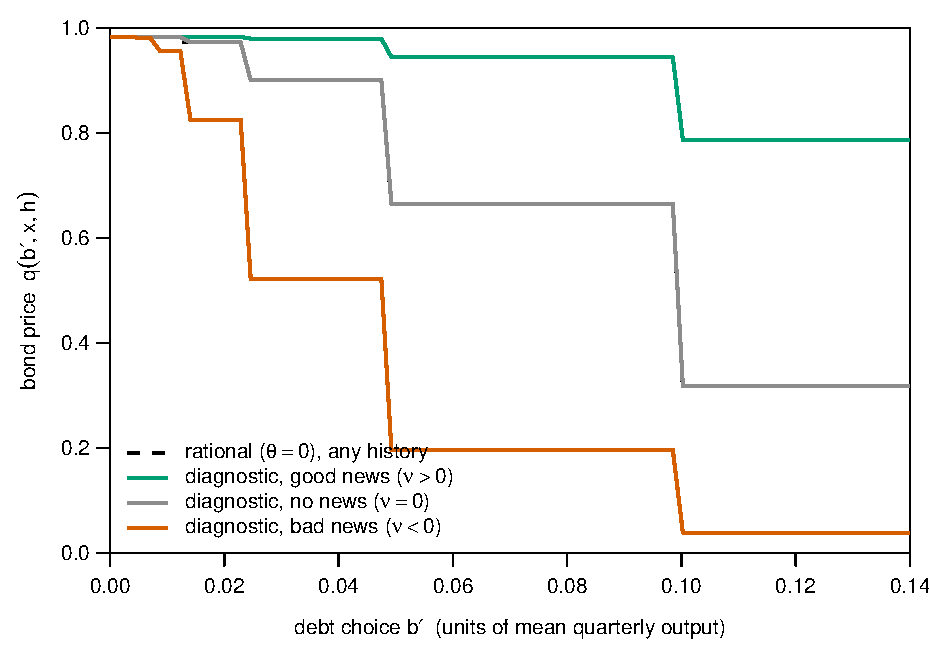
\includegraphics[width=0.72\textwidth]{fig_price.pdf}
\caption{Bond price schedules at median income, $\theta = 0.5$, for three histories of news $\nu = x - h$ (good and bad news set $|\nu|$ to about 2.7 standard deviations of the quarterly innovation for visibility). The dashed curve is the rational schedule, common to all histories.}
\label{fig:price}
\end{figure}

Figure~\ref{fig:defaultset} translates prices into default behavior: it plots the smallest debt at which the sovereign defaults, as a function of income, for the same three histories. This is Proposition~\ref{prop:fragility} drawn. Between the good-news and bad-news cutoffs lies the fragility corridor: combinations of debt and income that are safe if the economy arrived on an upswing and default-inducing if it arrived on a downswing. A sovereign whose debt sits in the corridor is betting on the sign of the next quarter's news. The rational model collapses this corridor to the empty set.

\begin{figure}[t]
\centering
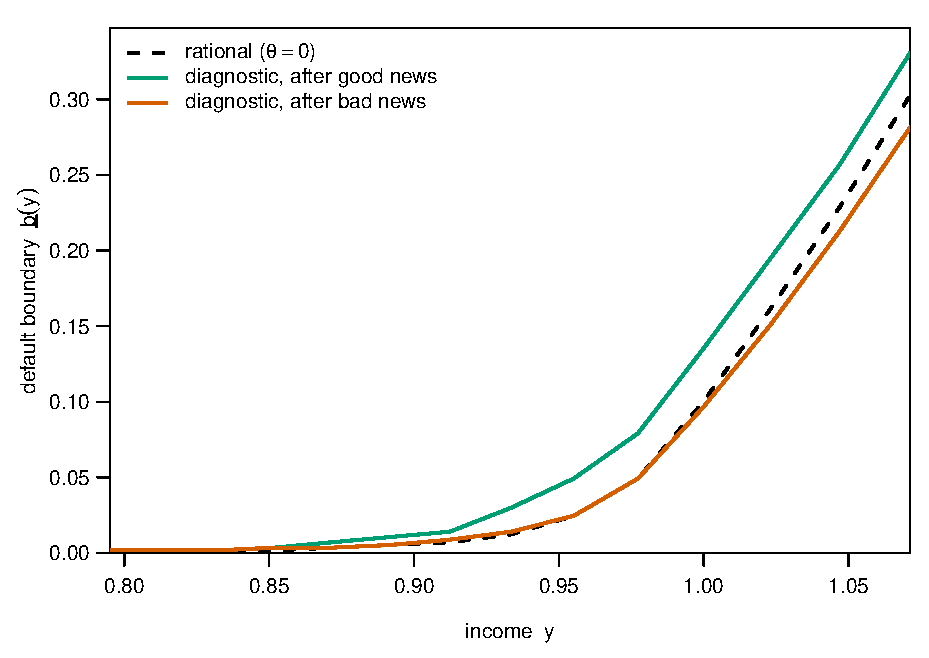
\includegraphics[width=0.72\textwidth]{fig_defaultset.pdf}
\caption{Default cutoffs $\underline{b}(y)$: the smallest debt triggering default, by income, $\theta = 0.5$. The region between the good-news and bad-news curves is history dependent.}
\label{fig:defaultset}
\end{figure}

\subsection{Simulated moments}

Table~\ref{tab:moments} reports moments from 500{,}000 simulated quarters under the \emph{true} income process, the same shock sequence for every $\theta$.

\begin{table}[t]
\centering
\caption{Simulated moments under the true income process.}
\label{tab:moments}
\begin{tabular}{lccc}
\toprule
 & $\theta = 0$ & $\theta = 0.5$ & $\theta = 1$ \\
\midrule
Median spread (percent, annualized) & \SprMedRE & \SprMedDiag & \SprMedOne \\
S.d.\ of spread (percent) & \SprSdRE & \SprSdDiag & \SprSdOne \\
Correlation of spread with log income & \CorrSprYRE & \CorrSprYDiag & \CorrSprYOne \\
Mean debt service to output (percent) & \DebtYRE & \DebtYDiag & \DebtYOne \\
Defaults per 100 years & \DefFreqRE & \DefFreqDiag & \DefFreqOne \\
Share of quarters with market access (percent) & \FracAccessRE & \FracAccessDiag & \FracAccessOne \\
News coefficient, within $(b', y)$ cells (bp per $1\sigma$) & \NewsBpRE & $\NewsBpDiag$ & $-$\NewsBpOneAbs \\
Implied forecast-revision coefficient $\beta_{CG}$ & 0 & \CGbetaHalf & \CGbetaOne \\
\bottomrule
\end{tabular}
\par\smallskip
\begin{minipage}{0.92\textwidth}
\footnotesize Notes: spreads are annualized from one-period bond prices and winsorized at the 1st and 99th percentiles before computing means and standard deviations. Medians are unaffected. The news coefficient is the slope of the winsorized spread on $\nu$ after demeaning both within cells defined by the debt choice and the income state, scaled by one standard deviation of $\nu$. It is the model analogue of a panel regression of spreads on forecast revisions with nonparametric controls for debt and output. All statistics condition on market access.
\end{minipage}
\end{table}

The news coefficient is zero to machine precision at $\theta = 0$. This is Corollary~\ref{cor:zero} holding in the simulated data, and the zero requires nonparametric conditioning. A linear regression of spreads on news with linear debt and output controls yields $\NewsBpRELin$ basis points per standard deviation in the \emph{rational} economy, an artifact of the spread schedule's curvature loading on the news term. At $\theta = 0.5$ the same linear specification even gets the sign wrong, because good news shifts issuance along the schedule. Within cells, the diagnostic economy prices news at $\NewsBpDiag$ basis points per standard deviation and the rational economy at zero. The empirical work in Section~\ref{sec:evidence} inherits this lesson directly: the news test must condition on debt and output flexibly, or it tests nothing.

The workhorse model's known weakness with one-period debt is that spreads are too stable. Diagnostic pricing multiplies the standard deviation of spreads by roughly \SprSdRatio\ while \emph{lowering} the median spread from \SprMedRE\ to \SprMedDiag\ percent. The economy spends most of its time calm, with compressed spreads, and occasionally explodes. Long quiet spells punctuated by crises emerge here from Gaussian shocks alone, outside disasters and regime switches.

The default frequency rises from \DefFreqRE\ to \DefFreqDiag\ per century, overshooting the 2--3 per century in Argentine data. I report this directly: the parameters outside beliefs were calibrated by \citet{Arellano2008} to hit the default frequency \emph{at} $\theta = 0$, so adding overreaction at fixed parameters raises it. Table~\ref{tab:moments} should therefore be read as comparative statics in $\theta$. Section~\ref{sec:recal} re-selects $(\beta, \phi)$ at the baseline value of $\theta$ and reports what survives, while the history-dependence results follow from Propositions~\ref{prop:history}--\ref{prop:fragility} at any parameter vector satisfying Assumption~\ref{ass:monotone}. The $\theta = 1$ column makes the fixed-parameter point in extreme form: at credit-cycle levels of overreaction the economy loses market access a quarter of the time, which is a warning in favor of re-estimating $\theta$ in each asset-class environment.

\subsection{Booms that end}

The model's dynamic content is easiest to see in an event study, and the simulation design allows a clean one: because the income path is exogenous and the shock sequence is common across $\theta$, I can locate every episode, \EventsN\ of them in half a million quarters, in which log income rises for at least three consecutive quarters and then falls, and compare the rational and diagnostic economies \emph{on the same episodes}. Figure~\ref{fig:boom} shows median spreads, mean debt, and the default hazard in event time.

\begin{figure}[t]
\centering
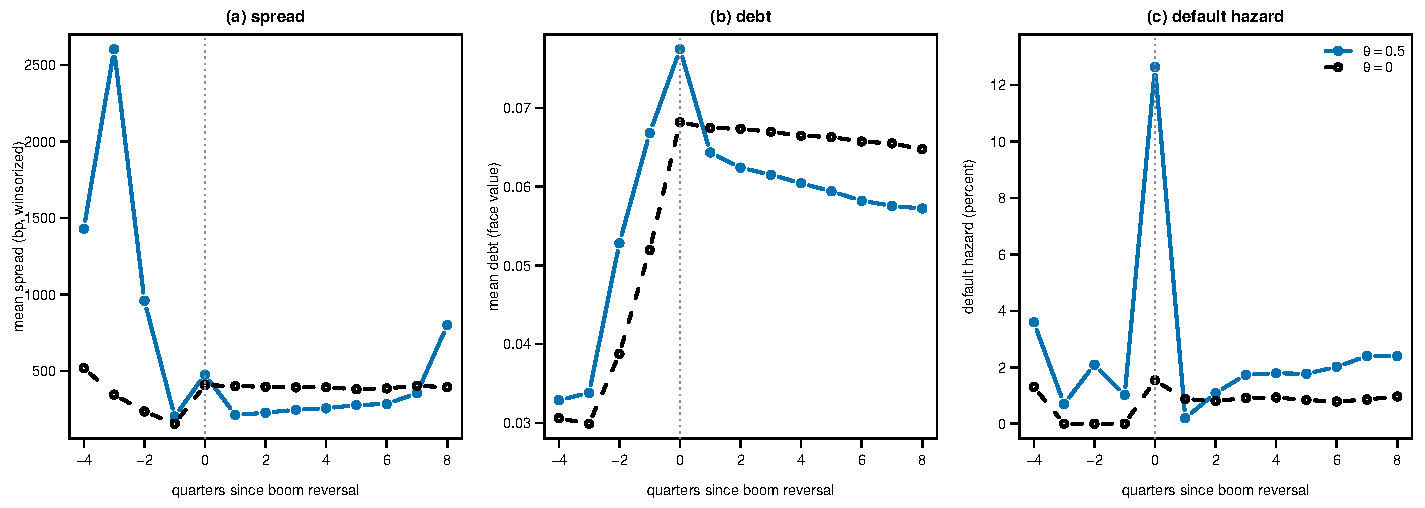
\includegraphics[width=\textwidth]{fig_boom.pdf}
\caption{Boom-reversal episodes: at least three consecutive rises in log income followed by a fall, identified on the common simulated income path (\EventsN\ episodes). Quarter 0 is the reversal. Spread and debt paths condition on continuous market access through the window. The default hazard is computed over the full risk set.}
\label{fig:boom}
\end{figure}

The figure shows the whole belief cycle. Entering the episode, on the heels of whatever bad news preceded the boom, the diagnostic economy pays spreads several times the rational level: pessimism is extrapolated too. The boom then compresses diagnostic spreads \emph{below} the rational benchmark, quarter by quarter, while debt rises by \BoomDebtRiseDiag\ percent against \BoomDebtRiseRE\ percent in the rational economy: the diagnostic sovereign borrows into the optimism, as the two-period example said it rationally should. The difference arrives with the reversal. In the quarter the news turns, the default hazard reaches \HazPeakDiag\ percent in the diagnostic economy, while on the identical income paths the rational economy's hazard is \HazPeakRE\ percent. The mechanics are exactly Propositions~\ref{prop:history} and \ref{prop:fragility} in sequence: the boom priced debt into the fragility corridor, and the first negative realization swings the belief tilt from extrapolated improvement to extrapolated decline, collapsing the price schedule and expanding the default set while debt is at its peak. Defaults follow booms in this model through fragile pricing created by the boom itself.

\subsection{Why two short-bond parameters do not constitute estimation}\label{sec:recal}

A two-parameter exercise is useful as a diagnostic and nothing more. At $\theta=0.5$, selecting $(\beta,\phi)$ to match three defaults per century and debt service of 5.5 percent gives $\beta=\BetaRecal$ and $\phi=\PhiRecal$. It restores those two moments. It also compresses the median spread to \SprMedRecal\ percent. The exercise cannot match default frequency, debt, spread levels, spread volatility, maturity, and returns with two free numbers. I therefore do not call it a recalibration of the diagnostic economy.

The diagnostic result that survives this deliberately narrow exercise is the conditional news effect. At the selected pair, the within-cell news coefficient is $-\NewsBpRecalAbs$ basis points per standard deviation and remains zero under rational pricing at the same parameters. The reversal-quarter hazards are \HazPeakRecalDiag\ percent and \HazPeakRecalRE\ percent. These figures show that the mechanism is not an artifact of the original short-bond parameter pair. Quantitative fit is assessed only in the long-duration simulated-moment exercise of Section~\ref{sec:longquant}.

Whether actual sovereign spreads behave this way is the next question.

\section{Evidence from Spreads and Forecasts}\label{sec:evidence}

The model makes four predictions that rational default pricing leaves at zero, each testable in a panel of emerging-market spreads matched to professional forecasts. Two organize the evidence. P1 uses the model's exact within-cell zero for news. P4 links the forecast estimate of $\theta_i$ to the spread response country by country. P2 and P3 describe the asymmetry and the return reversal that accompany the mechanism. Table~\ref{tab:feasibility} in Appendix~\ref{app:data} records the data sources, their coverage, and the replication files built from them.

\medskip
\noindent\textbf{P1 (decisive): news moves spreads conditional on fundamentals.} The estimating equation, at country $i$ and month $t$,
\begin{equation}
s_{i,t} \,=\, \alpha_{c(i,t)} + \tau_t + \delta\, \mathrm{Rev}_{i,t} + \Gamma' Z_{i,t} + e_{i,t},
\label{eq:spreadpanel}
\end{equation}
regresses the EMBI stripped spread on the consensus forecast revision of twelve-month-ahead real growth, where $\alpha_{c(i,t)}$ denotes fixed effects for \emph{cells} of debt-to-GDP and output relative to trend (country-specific bins), $\tau_t$ absorbs global conditions including the VIX and United States rates, and $Z$ holds the forecast \emph{level}, ratings, a country-specific commodity terms-of-trade index, and the revision of the consensus fiscal-balance forecast, so that the coefficient isolates income news from commodity news and fiscal news. Two features come straight from the theory. The cell fixed effects implement the nonparametric conditioning that Table~\ref{tab:moments} shows is necessary: with linear controls the rational benchmark moves away from zero and the test loses its interpretation. And the forecast level belongs in $Z$ because any rational model in which spreads respond to expected future income, such as \citet{AguiarGopinath2006} with trend shocks, makes the level informative. It is the \emph{revision}, conditional on the level, that overreaction prices. The model's magnitude at $\theta = 0.5$ is \NewsBpDiagAbs\ basis points per standard deviation of news at the comparative-static parameters and \NewsBpRecalAbs\ at the recalibrated ones, and the rational prediction is zero at both. Sticky-information models predict the opposite sign for consensus data, which makes the test three-cornered rather than one-sided.

\medskip
\noindent\textbf{P2 (supporting): the effect is asymmetric and strongest near the boundary.} Within the model, splitting $\nu$ into positive and negative parts gives within-cell responses of $-$\AsymPosDiag\ and $-$\AsymNegDiag\ basis points per standard deviation respectively, and interacting news with debt raises the response where debt is high. In the data this is \eqref{eq:spreadpanel} with $\mathrm{Rev}^+$, $\mathrm{Rev}^-$, and $\mathrm{Rev} \times \mathrm{Debt}$ terms. Winsorization mutes the crash tail in the model statistics, so the model's pooled asymmetry is a conservative benchmark.

\medskip
\noindent\textbf{P3 (supporting): returns reverse.} Proposition~\ref{prop:returns} predicts that EMBI excess returns are low following positive revisions and high following negative ones, conditional on spreads themselves: the sovereign analogue of \citet{GreenwoodHanson2013}. The regression of cumulative twelve-month excess returns on current revision histories, with the spread level controlled, has the rational null of zero once more. Risk-based stories require the \emph{price} of risk to fall exactly when sentiment measures say optimism reigns, which is testable by adding conventional risk-premium proxies.

\medskip
\noindent\textbf{P4 (decisive): the belief parameter travels.} Estimating $\theta_i$ country by country from forecasts (Section~\ref{sec:emdesign}) and the news coefficient $\delta_i$ country by country from \eqref{eq:spreadpanel} gives a cross-sectional restriction: $\delta_i$ should be increasing in $\theta_i$, and countries whose forecasters show overreaction near zero should show news effects near zero. This restriction is the paper's cleanest guard against a spread regression masquerading as a belief test, because the two panels are estimated separately.

\begin{table}[t]
\centering
\caption{Empirical predictions.}
\label{tab:evidence}
\begin{tabular}{p{4.6cm}p{3.4cm}p{3.2cm}p{2.4cm}}
\toprule
Test & Rational null & Model at $\theta=0.5$ & Estimation \\
\midrule
P1: within-cell news coefficient & 0 & $\NewsBpDiag$ bp per $1\sigma$ & EMBI and forecasts \\
P2: asymmetry, interaction with debt & 0, 0 & $-$\AsymPosDiag\ / $-$\AsymNegDiag\ bp & EMBI and forecasts \\
P3: return predictability from news & 0 & negative after booms & EMBI returns \\
P4: $\delta_i$ increasing in $\theta_i$ & flat relation & positive relation & country estimates \\
CG regression, individual forecasts & 0 & \CGbetaHalf & published for US\textsuperscript{a} \\
\bottomrule
\end{tabular}
\par\smallskip
\begin{minipage}{0.95\textwidth}
\footnotesize Notes: \textsuperscript{a}\citet{BordaloGennaioliMaShleifer2020} report negative individual-level forecast-error-on-revision coefficients for most United States macroeconomic series. The emerging-market estimation is specified in Section~\ref{sec:emdesign}. Data requirements: J.P.~Morgan EMBI Global stripped spreads (Bloomberg or Datastream), Consensus Economics individual forecaster panel, IMF WEO vintages, CBOE VIX, sovereign ratings. Table~\ref{tab:feasibility} records access and replication files.
\end{minipage}
\end{table}

Table~\ref{tab:evidence} collects the designs. Suppose they pass, and news moves sovereign spreads the way diagnostic pricing says. What, if anything, should a government do about it?

\section{Fiscal Rules under Diagnostic Pricing}\label{sec:rules}

The instrument I study is the simplest one in the policy debate: a ceiling $\bar b$ on debt issuance, imposed permanently and known to all parties. For each ceiling on a grid I recompute the full equilibrium, price schedule included, and evaluate welfare as the value at zero debt and median income \emph{under the true income process}, converting differences to basis points of permanent consumption. Because Section~\ref{sec:example} taught that the answer turns on whose beliefs are distorted, I compute the complete two-by-two: government rational or diagnostic, market rational or diagnostic, with $\theta = 0.5$ wherever beliefs are diagnostic. A diagnostic government maximizes under its own tilted kernel (the Bellman equations are in Appendix~\ref{app:extensions}), and its welfare is then evaluated under the truth. Everything in this section is a numerical property of computed equilibria at the baseline calibration, conditional on that welfare criterion. Figure~\ref{fig:rule} plots the welfare gain of each ceiling in each cell, and Table~\ref{tab:rules} reports the best ceiling per cell.

This criterion is sovereign welfare. Lender welfare is a different object. Competition makes expected profits zero under lenders' subjective law, not under the true law. I evaluate their true expected payoff from each issued bond and report the predictable excess returns separately. Global welfare would add sovereign utility, lender utility, output destroyed in default, and any international spillovers after placing them in common units. The baseline does not specify foreign marginal utility or spillovers, so it does not rank policies by global welfare. Every policy statement below concerns sovereign welfare under the true probability measure. A ceiling that benefits the sovereign may harm lenders, and the reverse may occur.

\begin{figure}[t]
\centering
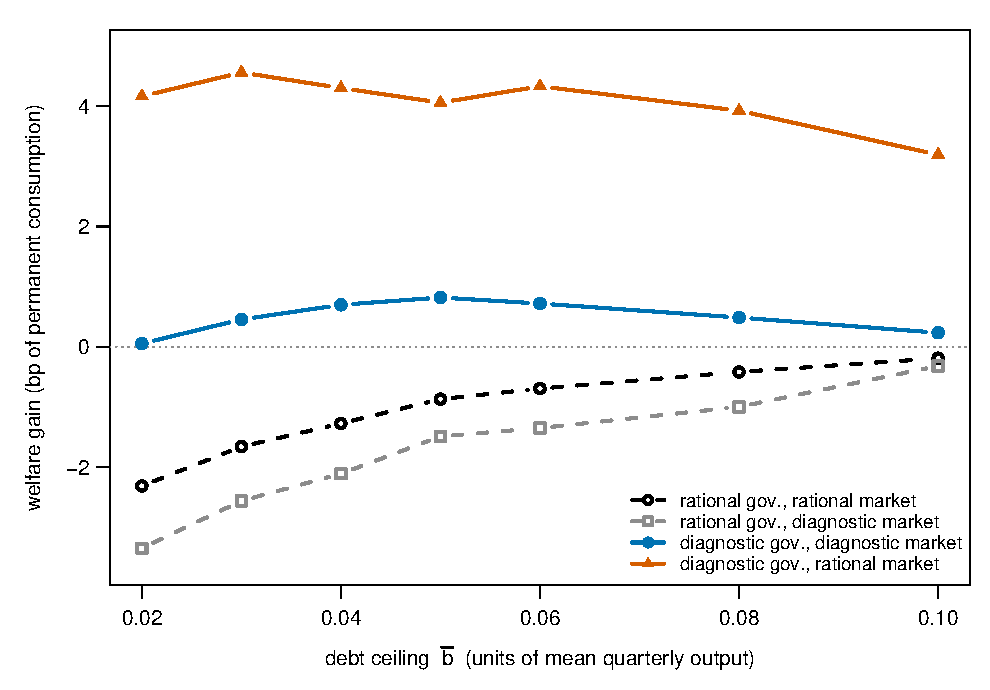
\includegraphics[width=0.78\textwidth]{fig_rule.pdf}
\caption{Welfare effect of a permanent debt ceiling $\bar b$, by configuration of beliefs, evaluated under the true income process at zero debt and median income. $\theta = 0.5$ where diagnostic.}
\label{fig:rule}
\end{figure}

\begin{table}[t]
\centering
\caption{The whose-beliefs two-by-two: welfare gain of the best debt ceiling.}
\label{tab:rules}
\begin{tabular}{lcc}
\toprule
 & Market rational & Market diagnostic \\
\midrule
Government rational & \CEbestA\ bp & \CEbestB\ bp \\
Government diagnostic & +\CEbestD\ bp & +\CEbestC\ bp \\
\bottomrule
\end{tabular}
\par\smallskip
\begin{minipage}{0.8\textwidth}
\footnotesize Notes: basis points of permanent consumption, at the best ceiling on the grid $\{0.02, \ldots, 0.10\}$ per cell. Negative entries mean every ceiling on the grid lowers welfare. $\theta = 0.5$ in diagnostic cells.
\end{minipage}
\end{table}

The sign pattern is the result. When the government is rational, every ceiling hurts, and it hurts \emph{more} when the market is diagnostic (\CEworstB\ basis points at the tightest ceiling, against \CEworstA\ in the fully rational cell): the rational government was selling overpriced debt to optimists, and the rule takes the trade away. When the government is diagnostic, ceilings help. Facing a diagnostic market the best ceiling yields $+$\CEbestC\ basis points and cuts the default frequency from \DefFreqCellC\ to \DefFreqCellCopt\ per century. Facing a rational market it yields $+$\CEbestD. The gains are largest in the cell where the market is rational because there the government's extrapolation earns zero offsetting rents: rational lenders price the optimistic government's future behavior correctly, so its overborrowing (mean debt service \DebtYCellD\ percent of output, against \DebtYRE\ in the rational benchmark) is pure loss, and the rule claws much of it back. Note also the diagnostic-government economies confirm the boom-overborrowing channel the two-period example leaves to the dynamic model: with persistent income, a government that extrapolates good news borrows against an expected future that disappoints, which is precisely the borrowing a good-news-contingent constraint would target.

The magnitudes are small, single basis points of permanent consumption, for the usual reason: in the one-period economy default's resource cost is modest and consumption smoothing is cheap. The long-duration calibration in Section~\ref{sec:quant} adds debt dilution to the positive analysis. A welfare exercise with long debt would add a second policy margin and is not needed for the sign result established here. The lesson itself is clean: \emph{under one-period debt, a benevolent government, and the computed equilibria at $\theta = 0.5$, a debt ceiling lowers sovereign welfare when the government prices the future correctly and raises it when the government extrapolates}. In this environment fiscal rules are a commitment device against the government's own extrapolation rather than a correction of market mispricing. The state variable the model identifies, the run of recent news, is observable in real time from forecast revisions, so a rule that tightens after sustained upward revisions is the natural state-contingent version of the flat ceiling studied here.

\section{Conclusion}\label{sec:conclusion}

I have taken the workhorse model of sovereign default and replaced one primitive, lenders' probability law. The degree of overreaction is measured from forecasts rather than fitted to bond prices. The cost is one observable pricing state. The return is a set of restrictions. Prices depend on recent news conditional on debt and output. True expected bond returns are low after good news. Default regions expand when optimism reverses. The one-period model establishes these results sharply. The long-duration implementation adds dilution, coupons, and capital gains and is the model used for quantitative fit. Each prediction has an estimating equation. The central empirical restriction is the within-cell news coefficient. A coefficient of zero after flexible conditioning on debt, output, expected growth, and fiscal news rejects the diagnostic channel in this environment.

The normative lesson runs against a common intuition. It is tempting to argue that if markets misprice sovereign risk, governments should be insulated from the market's moods by fiscal rules. The model says nearly the reverse: a rational government profits from the market's moods, and rules bind usefully only when the government shares them. Whether official decision makers share private forecast errors is therefore a separate empirical question. If they do, the argument for rules is about the state's own psychology, and the debate should be had on that ground.

The maintained environment is the sovereign-debt core used throughout the quantitative section. The government payoff is the planner payoff, lenders are risk neutral, and debt lasts one quarter. These choices make spreads map directly into default probabilities and make welfare comparisons consumption-equivalent values inside the Bellman system. The return tests in Section~\ref{sec:evidence} separate probability movements from risk premia in the data, while the extensions below show how government beliefs and long-duration bonds enter the same recursion.

Long-duration bonds put diagnostic booms and dilution into the same state variable. Risk-averse lenders would let forecast data separate time-varying risk premia from belief distortions. Country-level estimates of $\theta_i$ from the forecasters who price these bonds would turn the belief parameter into a measured input. The model stands on that number, which is where a theory of beliefs ought to stand.

\clearpage
\appendix
\renewcommand{\theequation}{\thesection.\arabic{equation}}
\numberwithin{equation}{section}

\section{Proofs}\label{app:proofs}

\subsection{Proof of Lemma \ref{lem:tilt}}
Write $m_x=\rho x$ and $m_h=\rho h$. Substituting the two Gaussian densities into \eqref{eq:diagnostic} gives the unnormalized exponent
\[
 -\frac{(1+\theta)(x'-m_x)^2-\theta(x'-m_h)^2}{2\sigma_\varepsilon^2}.
\]
Define $m_\theta=(1+\theta)m_x-\theta m_h$. Expanding both squares and collecting terms yields
\[
\begin{aligned}
&(1+\theta)(x'-m_x)^2-\theta(x'-m_h)^2\\
&\qquad=x'^2-2m_\theta x'+(1+\theta)m_x^2-\theta m_h^2\\
&\qquad=(x'-m_\theta)^2+(1+\theta)m_x^2-\theta m_h^2-m_\theta^2.
\end{aligned}
\]
The last three terms do not depend on $x'$, so the normalizing constant removes them. The normalized density is therefore
\[
\hat p_\theta(x'\mid x,h)
=\frac{1}{\sqrt{2\pi\sigma_\varepsilon^2}}
\exp\!\left[-\frac{(x'-m_\theta)^2}{2\sigma_\varepsilon^2}\right].
\]
Finally,
\[
m_\theta=(1+\theta)\rho x-\theta\rho h
=\rho x+\theta\rho(x-h),
\]
which proves the stated mean and variance. $\blacksquare$

\subsection{Proof of Proposition \ref{prop:existence}}
Let $\mathcal S$ be the finite set of market-access and exclusion states. For each market-access state $s\in\mathcal S$, let $\mathcal A(s)$ contain default and every debt-grid choice. Utility below the consumption floor is extended by the tangent at the floor. This extension is finite, continuous, strictly increasing, and agrees with CRRA utility above the floor. The product of the mixed-action simplexes,
\[
\Sigma=\prod_{s\in\mathcal S}\Delta(\mathcal A(s)),
\]
is nonempty, compact, and convex. The price set
\[
\mathcal Q=[0,1/R]^{|\mathcal B||\mathcal X|^2}
\]
has the same three properties.

Fix a price vector $q\in\mathcal Q$. The government's problem is a finite discounted Markov decision problem. Current utility is bounded on the finite action-state set, the transition matrix is stochastic, and $0<\beta<1$. Its Bellman operator is therefore a contraction in the sup norm with modulus $\beta$, so it has a unique value vector $V(q)$. Because every action value is a finite sum of continuous functions of $q$ and $V(q)$, the value vector is continuous in $q$. At each state, the set of optimal mixed actions is the simplex supported on the maximizing pure actions. The product correspondence $\Gamma(q)\subseteq\Sigma$ is consequently nonempty, compact, convex valued, and upper hemicontinuous.

For a mixed stationary policy $\sigma\in\Sigma$, let $P(\sigma)\in\mathcal Q$ be the zero-profit price vector. Each component is $1/R$ times a finite sum of diagnostic transition probabilities multiplied by the next-state mixed repayment probability. The map $P$ is linear in $\sigma$ and hence continuous.

Define the correspondence on $\mathcal Q\times\Sigma$ by
\[
\mathcal F(q,\sigma)=\{P(\sigma)\}\times\Gamma(q).
\]
Its domain is nonempty, compact, and convex. Its values are nonempty, compact, and convex. Continuity of $P$ and upper hemicontinuity of $\Gamma$ imply that $\mathcal F$ is upper hemicontinuous. Kakutani's fixed-point theorem therefore gives $(q^*,\sigma^*)\in\mathcal F(q^*,\sigma^*)$. The policy $\sigma^*$ is optimal at $q^*$ and $q^*$ satisfies zero profit under $\sigma^*$, which is a stationary recursive equilibrium in mixed policies. If a computed deterministic policy has zero Bellman and pricing residuals, its degenerate mixed representation satisfies the same two conditions in the extended economy. If every repayment choice gives consumption above the floor, the extension is never used at an optimal action. The deterministic fixed point then solves the original positive-consumption problem. $\blacksquare$

\subsection{Proof of Lemma \ref{lem:fosd}}
By Lemma~\ref{lem:tilt}, $F_\theta(\cdot \mid x, h_i)$ is the Gaussian cdf with variance $\sigma_\varepsilon^2$ and mean $\mu_i = \rho x + \theta \rho \nu_i$. For $\nu_2 > \nu_1$ and $\theta > 0$, $\mu_2 > \mu_1$, and a Gaussian family with common variance is strictly ordered by first-order stochastic dominance in its mean: $F(z - \mu)$ is decreasing in $\mu$ for every $z$. $\blacksquare$

\subsection{Proof of Lemma \ref{lem:bmono}}
Fix $(x,h)$ and debt levels $b_2>b_1$ in $\mathcal B$. If repayment is feasible at $b_2$, compactness of $\mathcal B$ and continuity on the feasible set give a maximizing issuance choice $b_2'$. Consumption from that same choice at $b_1$ exceeds consumption at $b_2$ by $b_2-b_1>0$. The continuation value is unchanged because it depends on $b_2'$ and $(x,h)$ but not on inherited debt. Strict monotonicity of $u$ therefore gives
\[
\begin{aligned}
V^R(b_1,x,h)
&\geq u\big(y+q(b_2',x,h)b_2'-b_1\big)
  +\beta\E[V(b_2',x',x)\mid x]\\
&>u\big(y+q(b_2',x,h)b_2'-b_2\big)
  +\beta\E[V(b_2',x',x)\mid x]\\
&=V^R(b_2,x,h).
\end{aligned}
\]
If repayment is infeasible at $b_2$, default is forced and the upper-set conclusion already holds at that debt. The default value in \eqref{eq:vd} is independent of inherited debt. Hence $d=\one\{V^D>V^R\}$ is nondecreasing in $b$, and the default set is an upper interval. $\blacksquare$

\subsection{Proof of Proposition \ref{prop:history} and Corollary \ref{cor:zero}}
Fix $(b', x)$ and write $g(x') = 1 - d(b', x', x)$, the repayment indicator next period. Under Assumption~\ref{ass:monotone}, $g$ is nondecreasing. From \eqref{eq:price}, $R\, q = \int g \, dF_\theta(\cdot \mid x, h)$. If $\nu_2 > \nu_1$, Lemma~\ref{lem:fosd} gives first-order dominance, and the expectation of a nondecreasing function is nondecreasing under first-order dominance. Hence $q$ is nondecreasing in $\nu$.

For strictness, suppose $\theta > 0$ and default risk is interior at $(b', x)$: $0 < \int g\, dF_\theta < 1$. Because income is Markov on a totally ordered set and $g$ is a nondecreasing indicator, interiority means $g$ switches from $0$ to $1$ at some finite threshold $\underline{x}'(b', x)$ in the interior of the support. Writing $Z \sim N(0, \sigma_\varepsilon^2)$,
\[
R\,q(\nu) = \E\big[\, g(\mu(\nu) + Z) \,\big] = \Prob\{ Z \ge \underline{x}' - \mu(\nu) \},
\]
with $\mu(\nu) = \rho x + \theta\rho \nu$ strictly increasing in $\nu$. Since the Gaussian distribution assigns positive density everywhere, the probability is strictly increasing in $\mu$. This proves the proposition.

For the corollary: at $\theta = 0$ the kernel $\hat p_0(\cdot \mid x, h) = p(\cdot \mid x)$ is independent of $h$, so $q$ is a function of $(b', x)$ alone and any statistic of $q$ computed within a $(b', x)$ cell has zero variation in $\nu$. Conversely, if $\theta > 0$ and default risk is interior at some $(b', x)$ visited with positive probability, the strict monotonicity just established makes the within-cell slope strictly negative for spreads (spreads are strictly decreasing transformations of $q$). $\blacksquare$

\subsection{Proof of Proposition \ref{prop:returns}}
A lender pays $q(b',x,h)>0$ and receives $g(x')=1-d(b',x',x)$. At fixed $(b',x)$, define $A=\E_p[g\mid x]$ and $B(\nu)=\E_{\hat p_\theta}[g\mid x,h]$. The true-measure expected excess gross return is
\[
R^e(\nu)=R\left(\frac{A}{B(\nu)}-1\right).
\]
The quantity $A$ does not depend on $\nu$. Proposition~\ref{prop:history} implies that $B(\nu)$ is positive and nondecreasing on the positive-price domain. Thus, if $\nu_2>\nu_1$, then $A/B(\nu_2)\leq A/B(\nu_1)$, so $R^e$ is nonincreasing. At $\theta=0$, the diagnostic and true kernels coincide, which gives $A=B$ and $R^e=0$. If $\theta>0$ and $\nu>0$, the diagnostic kernel first-order stochastically dominates the true kernel. Since $g$ is nondecreasing, $B(\nu)\geq A$ and $R^e\leq0$. For $\nu<0$, the true kernel dominates the diagnostic kernel, so $B(\nu)\leq A$ and $R^e\geq0$. The inequalities are strict when the repayment indicator changes on a set with positive diagnostic probability. $\blacksquare$

\subsection{Proof of Proposition \ref{prop:fragility}}
Take the equilibrium price schedule $q$ and continuation value as given, and compare two histories $\nu_2 > \nu_1$ at the same $(b, x)$. For every candidate issuance $b' \geq 0$, consumption $y + q(b', x, h)b' - b$ is nondecreasing in $\nu$ by Proposition~\ref{prop:history}, and the continuation $\E[V(b', x', x) \mid x]$ is independent of $h$ because the government's expectation is rational and tomorrow's reference is today's $x$. Hence each candidate's objective in \eqref{eq:vr} is nondecreasing in $\nu$, and $V^R$, a pointwise supremum of nondecreasing functions of $\nu$, is nondecreasing in $\nu$. $V^D$ in \eqref{eq:vd} involves neither $b$ nor $h$. Therefore $d = \one\{V^D > V^R\}$ is nonincreasing in $\nu$, which is the set inclusion claimed. $\blacksquare$

\subsection{Proof of Proposition \ref{prop:cg}}
Under the fixed-target convention, the diagnostic forecast of $x_{t+1}$ made at $t$ is $F_t x_{t+1} = \E_t x_{t+1} + \theta(\E_t x_{t+1} - \E_{t-1} x_{t+1})$ with $\E_t x_{t+1} = \rho x_t$ and $\E_{t-1} x_{t+1} = \rho^2 x_{t-1}$, so
\[
F_t x_{t+1} = \rho x_t + \theta \rho \varepsilon_t, \qquad
F_{t-1} x_{t+1} = \rho^2 x_{t-1} + \theta \rho^2 \varepsilon_{t-1}.
\]
Hence the revision and the error are
\[
\mathrm{Rev}_t = F_t x_{t+1} - F_{t-1} x_{t+1} = \rho(1+\theta)\varepsilon_t - \theta\rho^2 \varepsilon_{t-1},
\qquad
\mathrm{FE}_{t+1} = x_{t+1} - F_t x_{t+1} = \varepsilon_{t+1} - \theta\rho\,\varepsilon_t .
\]
The innovations are i.i.d., so
\[
\operatorname{Cov}(\mathrm{FE}_{t+1}, \mathrm{Rev}_t) = -\theta(1+\theta)\rho^2 \sigma_\varepsilon^2,
\qquad
\operatorname{Var}(\mathrm{Rev}_t) = \rho^2 \sigma_\varepsilon^2\big[(1+\theta)^2 + \theta^2\rho^2\big],
\]
and the ratio is \eqref{eq:cgmap}. The same algebra at horizon $k$ for a fixed target $x_{t+k}$ gives $\mathrm{Rev}=\rho^k(1+\theta)\varepsilon_t-\theta\rho^{k+1}\varepsilon_{t-1}$ and $\mathrm{FE}=\sum_{j=1}^{k}\rho^{k-j}\varepsilon_{t+j}-\theta\rho^k\varepsilon_t$. The coefficient is horizon invariant for that fixed-target experiment. Annual fixed-event forecasts combine targets and calendar weights. They require the simulation mapping in Section~\ref{sec:emdesign}. $\blacksquare$

\section{The Two-Period Example: Details}\label{app:example}

Consumption at date 0 is $c_0 = y_0 + qb$ with $q = \hat\pi / R$ in the risky region $\psi y_L < b \leq \psi y_H$. The objective is $\ln c_0 + \beta[\pi \ln(y_H - b) + (1-\pi) \ln((1-\psi) y_L)]$, and only the first two terms involve $b$. The first-order condition is
\[
\frac{\hat\pi / R}{y_0 + (\hat\pi/R) b} \,=\, \frac{\beta \pi}{y_H - b},
\]
and solving the linear equation gives \eqref{eq:bstar}. Differentiating \eqref{eq:bstar} in $\hat\pi$ gives $\partial b^*/\partial \hat\pi = \beta \pi R y_0 / [\hat\pi^2 (1+\beta\pi)] > 0$. The second-order condition holds by concavity in $b$.

\paragraph{The safe--risky margin.} The best safe plan solves $\max_{b \leq \psi y_L} \ln(y_0 + b/R) + \beta[\pi \ln(y_H - b) + (1-\pi)\ln(y_L - b)]$ and its value $W^{S}$ is independent of $\hat\pi$. The best risky plan's value $W^{R}(\hat\pi)$ is strictly increasing in $\hat\pi$ by the envelope theorem, since $\partial W^R/\partial \hat\pi = u'(c_0)\, b^*/R > 0$. If parameters are such that $W^R(\pi) < W^S < \lim_{\hat\pi \to 1} W^R(\hat\pi)$, there is a threshold $\hat\pi^\dagger$ at which the sovereign switches from safe to risky borrowing, and optimism beyond the threshold raises the true default probability from $0$ to $1 - \pi$ discontinuously.

\paragraph{A diagnostic government in the example.} If the government also prices the future with $\hat\pi$, the first-order condition becomes $(\hat\pi/R)/c_0 = \beta \hat\pi\, u'(y_H - b)$, in which $\hat\pi$ cancels from the price side and the belief side:
\[
\hat b \,=\, \frac{y_H - \beta R y_0}{1 + \beta \hat\pi},
\]
which is \emph{decreasing} in $\hat\pi$. Probability optimism makes repayment subjectively more likely and so subjectively more expensive, and with log utility this cost effect outweighs the price effect. The example is therefore the probability-optimism case. In the infinite-horizon model, optimism is about the \emph{level} of future income, and the consumption-smoothing motive of an optimist is to borrow against the good future it expects. Quantitatively that channel dominates, and mean debt in the diagnostic-government cells exceeds the rational benchmark (Section~\ref{sec:rules}). The contrast disciplines the interpretation of two-period intuition in this class of models.

\section{Computation}\label{app:computation}

\paragraph{Discretization.} Log income uses a \citet{Tauchen1986} chain with $n_x = 21$ states spanning $\pm 3$ unconditional standard deviations. The diagnostic kernel is discretized by the same binning rule applied to the $N(\rho x_i + \theta\rho(x_i - x_k),\, \sigma_\varepsilon^2)$ density for every pair $(i, k)$, which is exact up to the binning because Lemma~\ref{lem:tilt} keeps the tilted density Gaussian with unchanged variance. Debt lives on an evenly spaced grid of $n_b = 200$ points on $[0, 0.35]$ in units of mean quarterly output.

\paragraph{Algorithm.} Given a price array $q$, one backward-induction sweep updates $V^D$, $V^R$ (by full maximization over the debt grid), $V$, and $d$. The price is then updated from \eqref{eq:price} and damped, $q \leftarrow \tfrac12 q + \tfrac12 q^{\text{new}}$. The joint iteration runs to $\sup$-norm tolerances of $5 \times 10^{-8}$ on both $V$ and $q$, reached in 351 iterations at every $\theta$, and a full solve takes roughly twenty seconds in multithreaded Julia on a laptop. At $\theta = 0$ the computed equilibrium reproduces the \citet{Arellano2008} benchmark by construction.

\paragraph{Simulation.} 500{,}000 quarters after a 1{,}000-quarter burn-in, with the income path drawn once and reused across every configuration (common random numbers), so that cross-$\theta$ comparisons and the event study condition on identical fundamentals. Statistics condition on market access. Spreads are annualized from quarterly prices and winsorized at the 1st and 99th percentiles for means and standard deviations.

\paragraph{Survey mapping.} The monthly validation uses \SurveyMonths\ simulated months. At each date the code constructs current-year and next-year annual-average growth forecasts, converts them to a rolling twelve-month forecast with the empirical calendar weights, and estimates the same forecast-error regression used on the data. The map is evaluated on a grid of $\theta$ values and inverted by monotone bisection. Inputs $\theta\in\{0,0.25,0.5,1\}$ are recovered within 0.02. At the baseline, the recovery error is \SurveyRecoveryError.

\paragraph{Verification of Assumption \ref{ass:monotone} and grid robustness.} In the computed equilibria at $\theta \in \{0, 0.5\}$ income-monotonicity and the debt-monotonicity that Lemma~\ref{lem:bmono} guarantees hold across all grid combinations. At $\theta = 1$ a small fraction of grid columns shows a violation at extreme states with near-degenerate pricing: 0.02 percent at the baseline grids and \MonoViolGDOnepct\ percent at doubled grids. Doubling both grids ($n_x = 31$, $n_b = 400$) gives zero violations at $\theta \in \{0, 0.5\}$. Replacing the asymmetric default cost with a proportional cost $y^D = (1-\psi)y$ for $\psi \in \{0.02, 0.05\}$ gives zero violations. All thirty parameter vectors visited by the recalibration search, and the recalibrated final pair, satisfy both monotonicities at every grid point. The headline moments are also stable under grid doubling: at $\theta = 0.5$ the within-cell news coefficient moves from \NewsBpDiag\ to $-$\NewsBpDiagGD\ basis points per standard deviation, the default frequency from \DefFreqDiag\ to \DefFreqDiagGD\ per century, and the reversal-quarter hazard from \HazPeakDiag\ to \HazPeakDiagGD\ percent (\HazPeakRE\ to \HazPeakREGD\ for the rational economy), while the rational news coefficient remains zero (\NewsBpREGD). The winsorized spread standard deviation is visibly grid-sensitive (\SprSdDiag\ against \SprSdDiagGD\ percent), as it inherits the extreme spread tail. The volatility ratio to the rational economy remains far above one at both densities, and the paper's conclusions use the news coefficient, default frequency, and reversal hazard.

\paragraph{Short-bond diagnostic grid.} The grid behind Section~\ref{sec:recal} is
\[
\beta\in\{0.945,0.953,0.961,0.969,0.977\},
\qquad
\phi\in\{0.880,0.895,0.910,0.925,0.945,0.969\}.
\]
Each pair is solved at $\theta=0.5$ and simulated for 200{,}000 quarters. The calculation asks whether two short-bond parameters can restore default frequency and debt service. It is not the estimation criterion used for the long-duration model.

\begin{table}[t]
\centering
\caption{Parameter discipline and sensitivity.}
\label{tab:params}
\scriptsize
\setlength{\tabcolsep}{2pt}
\begin{tabular}{p{1.8cm}p{1.8cm}p{2.0cm}p{2.8cm}p{1.9cm}p{3.0cm}}
\toprule
Parameter & Units, frequency & Category & Source or target (sample) & Range examined & Effect on headline results \\
\midrule
$\gamma = 2$, eq.~\eqref{eq:vr} & dimensionless & externally fixed & standard value in the quantitative default literature & fixed & scales welfare units, signs fixed \\
$\beta = 0.953$, eq.~\eqref{eq:vr} & quarterly & internally calibrated & default moments at $\theta = 0$ \citep{Arellano2008}, re-selected at $\theta = 0.5$: \BetaRecal & 0.945--0.977 & default frequency falls steeply in $\beta$ (14.2 to 1.0 per century across the grid) \\
$r^* = 0.017$, eq.~\eqref{eq:price} & quarterly & externally fixed & U.S. five-year yield \citep{Arellano2008} & fixed & shifts spread levels one for one \\
$\rho = 0.945$, eq.~\eqref{eq:ar1} & quarterly & directly estimated & detrended Argentine real GDP \citep{Arellano2008} & mapping check & $\beta_{CG}(\theta)$ mapping nearly flat in $\rho$, tilt size scales with $\theta\rho$ \\
$\sigma_\varepsilon = 0.025$, eq.~\eqref{eq:ar1} & quarterly & directly estimated & detrended Argentine real GDP \citep{Arellano2008} & fixed & scales news size, signs fixed \\
$\lambda = 0.282$, eq.~\eqref{eq:vd} & quarterly & externally fixed & market re-access delays \citep{Arellano2008} & fixed & shortens exclusion, lowers effective default cost \\
$\phi = 0.969$, eq.~\eqref{eq:vd} & fraction of $\E[y]$ & internally calibrated & spread moments at $\theta = 0$ \citep{Arellano2008}, re-selected at $\theta = 0.5$: \PhiRecal & 0.880--0.969 & governs default frequency and debt capacity jointly with $\beta$ \\
$\theta = 0.5$, eq.~\eqref{eq:diagnostic} & dimensionless & baseline in published range & individual CG regressions \citep{BordaloGennaioliMaShleifer2020}, EM estimate in Section~\ref{sec:emdesign} & $\{0, 0.25, 0.5, 1\}$ & mechanism vanishes exactly at $\theta = 0$, market access collapses near $\theta = 1$ at fixed $(\beta,\phi)$ \\
\bottomrule
\end{tabular}
\par\smallskip
\begin{minipage}{0.97\textwidth}
\footnotesize Notes: categories follow the four-way scheme of Section~\ref{sec:quant}. Validation uses moments separate from calibration: the within-cell news coefficient, the return-predictability pattern, and the boom-reversal hazard profile all stay outside the calibration and recalibration loss. The region where the mechanism disappears is stated explicitly: all history dependence vanishes at $\theta = 0$, continuously, and the environment stops resembling emerging-market data near $\theta = 1$ at fixed parameters outside beliefs.
\end{minipage}
\end{table}

\paragraph{Welfare.} Consumption equivalents between configurations use $\Delta = (W_1 / W_0)^{1/(1-\gamma)} - 1$ evaluated at zero debt and median income under the true measure. For diagnostic-government cells $W$ is computed by policy evaluation as in Appendix~\ref{app:extensions}.

\section{Data Appendix}\label{app:data}

\paragraph{Spreads.} J.P.~Morgan EMBI Global stripped spreads, by country, monthly averages of daily quotes, accessed through Bloomberg or Datastream. The stripped spread nets out collateralized cash flows and is the standard market-risk measure in this literature \citep{UribeYue2006, LongstaffEtAl2011}. Spreads are winsorized at the 1st and 99th percentiles within country. Default and restructuring windows are coded using the \citet{CrucesTrebesch2013} episode list and excluded from pricing regressions, mirroring the model's conditioning on market access.

\paragraph{Forecasts.} Consensus Economics monthly surveys, individual-forecaster level, of real GDP growth for the current and next calendar year, available for the major emerging markets from the early-to-mid 1990s. Fixed-event forecasts are converted to a fixed twelve-month horizon by weighting the two events by months remaining in the year: $F^{12m}_t = \tfrac{m}{12} F^{y}_t + (1 - \tfrac{m}{12}) F^{y+1}_t$, with $m$ the months left in year $y$. Revisions are month-over-month changes in $F^{12m}$, and the fixed-target revisions used for the Coibion--Gorodnichenko regressions are computed within event year. Realized growth is the \emph{first-release} outturn from the IMF World Economic Outlook vintage database, so that forecast errors use the information set available before later data revisions.

\paragraph{Fundamentals and controls.} General government debt to GDP comes from the WEO, and output relative to trend from a country-specific quadratic trend in log real GDP (robustness: Hamilton filter). The CBOE VIX and the ten-year United States Treasury yield serve as global controls, absorbed by time effects in the baseline. Standard \& Poor's long-term foreign-currency ratings are mapped to a 21-notch scale. One timing mismatch deserves notice: WEO debt is annual, and interpolating it to monthly frequency puts measurement error inside the conditioning cells. The design therefore uses lagged debt for cell assignment to avoid look-ahead, and quarterly BIS debt data cover a subsample for robustness.

\paragraph{Sample.} The intersection of EMBI Global membership and Consensus coverage with at least ten years of joint data, roughly 25 countries including Argentina, Brazil, Bulgaria, Chile, China, Colombia, Ecuador, Hungary, Indonesia, Malaysia, Mexico, Nigeria, Panama, Peru, the Philippines, Poland, Russia, South Africa, Turkey, Ukraine, and Venezuela, monthly, 1994--2024. Cell fixed effects for \eqref{eq:spreadpanel} use country-specific terciles of debt-to-GDP crossed with terciles of output relative to trend, with finer bins as a robustness dimension. Standard errors are clustered two-way by country and month, with Driscoll--Kraay errors as robustness given overlapping forecast horizons.

\begin{table}[t]
\centering
\caption{Data and implementation.}
\label{tab:feasibility}
\footnotesize
\setlength{\tabcolsep}{4pt}
\begin{tabular}{p{3.2cm}p{2.8cm}p{1.7cm}p{2.1cm}p{2.0cm}p{1.8cm}}
\toprule
Dataset & Coverage & Frequency & Access & Observed or proxied & Replication \\
\midrule
EMBI Global stripped spreads (J.P.~Morgan) & $\sim$25 countries, 1994--2024 & daily, used monthly & Bloomberg or Datastream license & observed & code shareable, raw data licensed \\
Consensus Economics, individual forecasters & major emerging markets, mid-1990s--2024 & monthly & commercial license & observed & code shareable, raw data licensed \\
IMF WEO vintage database & all sample countries & semiannual vintages & public & observed & shareable \\
WEO debt to GDP & all sample countries & annual & public & interpolated to monthly (proxy) & shareable \\
S\&P foreign-currency ratings & all sample countries & event dates & licensed & mapped to 21-notch scale & derived series shareable \\
CBOE VIX, U.S. Treasury yields & global & daily & public & observed & shareable \\
\citet{CrucesTrebesch2013} restructurings & episodes, 1970--2013 & episode & public & observed & shareable \\
\bottomrule
\end{tabular}
\par\smallskip
\begin{minipage}{0.95\textwidth}
\footnotesize Notes: the binding inputs are the two licensed panels. Both are standard in the literature and available at the institutions where this work would be conducted. Replication files can include all code, all public data, and exact extraction instructions for the licensed series.
\end{minipage}
\end{table}

\section{Extensions}\label{app:extensions}

\subsection{The diagnostic government}\label{app:diaggov}

When the government itself holds diagnostic beliefs, its expectations in \eqref{eq:vr}--\eqref{eq:vd} are taken under $\hat p_{\theta_g}(\cdot \mid x, h)$, and the default value acquires the belief state: the Bellman system becomes
\begin{align}
V^R(b, x, h) &= \max_{b'} \Big\{ u\big(y + q(b',x,h)b' - b\big) + \beta \int V(b', x', x)\, \hat p_{\theta_g}(x' \mid x, h)\, dx' \Big\}, \\
V^D(x, h) &= u(y^D(x)) + \beta \int \big[ \lambda V(0, x', x) + (1-\lambda) V^D(x', x) \big]\, \hat p_{\theta_g}(x' \mid x, h)\, dx',
\end{align}
with lenders pricing under $\hat p_{\theta_\ell}$ as before. The formulation treats the government as sophisticated about its own future beliefs in the stationary sense: it correctly anticipates that its future self will evaluate continuation problems with the tilt implied by the future state $(x', x)$. Because the tilted kernel is Markov on $(x, h)$, the fixed point is well defined. The alternative, anticipated-utility formulation in which the government treats today's tilted forecast as permanent gives similar quantitative answers in related settings and is a robustness item. \emph{True} welfare of the induced policies $(d, b')$ solves the linear system
\[
W(b, x, h) = \begin{cases} W^D(x), & d(b,x,h) = 1,\\[2pt]
u\big(c(b,x,h)\big) + \beta \int W\big(b'(b,x,h), x', x\big)\, p(x' \mid x)\, dx', & d = 0,\end{cases}
\]
with $W^D$ defined analogously under $p$, and all welfare statements in Section~\ref{sec:rules} use $W$.

\subsection{Long-duration bonds}\label{app:longbonds}

The quantitative model uses the random-maturity bond of \citet{ChatterjeeEyigungor2012}. A fraction $\delta$ of each unit matures each quarter. The remaining fraction pays coupon $z$ and survives. If $b$ is debt at the start of the quarter and $b'$ is debt after issuance, repayment consumption is
\begin{equation}
c=y+m-\bigl[\delta+(1-\delta)z\bigr]b
+q(b',x,h)\bigl[b'-(1-\delta)b\bigr].
\label{eq:longbudget}
\end{equation}
The sovereign's repayment value is
\[
V^R(b,x,h,m)=\max_{b'\in\mathcal B}
\left\{u(c)+\beta Z(b',x)\right\},
\]
where
\[
Z(b',x)=\sum_{x'}P(x'\mid x)
\int V(b',x',x,m')\,dG(m').
\]
The temporary shock has a truncated normal distribution. It is independent over time and has standard deviation $0.003$, the value in \citet{ChatterjeeEyigungor2012}. Default in the current quarter resets it to the lower support point. During exclusion it is again drawn from $G$. The code therefore keeps separate the integrated exclusion value and the value used in the current default comparison. Numerical stability comes from continuation in $\theta$ and damping of the fixed-point map. No economic parameter is altered to obtain convergence.

Competitive lenders satisfy
\[
q(b',x,h)=\frac{1}{R}\Ehat_\theta\!\left[
\bigl(1-d(b',x',x,m')\bigr)
\left\{\delta+(1-\delta)\left[z+q\bigl(b''(b',x',x,m'),x',x\bigr)\right]\right\}
\mathrel{\Big|}x,h\right].
\]
Thus the risk-free price is $[\delta+(1-\delta)z]/(\delta+r^*)$. Setting $\delta=1$ removes the resale term and reproduces the one-period price and default arrays point for point in the numerical test.

The continuous shock is used as a computational regularization, as in the original paper. For every $(b,x,h)$, the algorithm recovers all thresholds at which the optimal debt choice changes. It integrates bond payoffs exactly over the associated probability masses. It integrates utility by twenty-node Gaussian quadrature within each fixed-policy interval. An adaptive quadrature calculation provides an independent accuracy check. The fixed-point objects are $Z$, the integrated exclusion value, and $q$. The value objects receive full Bellman updates, while prices use a damping weight of $0.99$. Continuation in $\theta$ is performed on a 12-node debt grid. The target solution at $\theta=0.5$ is then prolonged by linear interpolation to 50 debt nodes, where the original operator is resolved. The largest residual across the continuation, exclusion, and pricing equations is \LongFPResidual. Solutions started from the risk-free schedule and from the zero schedule agree in the low-resolution multiple-initialization audit. The one-period limit agrees exactly with the separate short-bond code. Deterministic-policy iteration cycles on some intermediate and finer debt grids because discrete choices switch at near ties. The finite-grid existence result allows mixing at such ties. I report the converged deterministic 50-node equilibrium and do not treat a failed deterministic iteration as an equilibrium.

The economic parameter block is taken as a block from \citet{ChatterjeeEyigungor2012}. It sets $\delta=0.05$, $z=0.03$, $r^*=0.01$, the re-entry probability to $0.0385$, and $\beta=0.95460$. The persistent income process has $\rho=0.948503$ and innovation standard deviation $0.027092$. The default loss is $\max\{0,d_0y+d_1y^2\}$ with $d_0=-0.18845$ and $d_1=0.24559$. These values were jointly selected in that paper to match mean debt, the mean spread, and spread volatility. The belief exercise holds this block fixed and changes only $\theta$. This is the controlled long-debt mechanism comparison. The estimation exercise fixes $\theta$ from forecasts and minimizes the reported simulated-moment loss over $(\beta,d_0,d_1)$.

\subsection{Reference-belief conventions}\label{app:conventions}

The model's reference density is $p(\cdot\mid h)$, the kernel evaluated at yesterday's state, which keeps the belief state two-dimensional and Lemma~\ref{lem:tilt} exact. \citet{BordaloGennaioliMaShleifer2020} define the reference as the lagged forecast of the same target, giving the tilted mean $\rho x+\theta\rho(x-\rho h)=\rho x+\theta\rho\varepsilon_t$. The two means differ by $\theta\rho(1-\rho)h$, about five percent of the tilt at the calibrated persistence. Every result in Section~\ref{sec:theory} goes through under the alternative convention with $\nu$ redefined as the innovation $\varepsilon$. The FOSD ordering in Lemma~\ref{lem:fosd} needs only a mean tilt increasing in news. The fixed-target horizon result in Proposition~\ref{prop:cg} does not by itself cover annual fixed-event forecasts. Section~\ref{sec:emdesign} supplies that mapping by simulation.

\subsection{Additional quantitative results}\label{app:addl}

At $\theta=1$ the one-period economy defaults \DefFreqOne\ times per century and holds market access only \FracAccessOne\ percent of the time. Median spreads collapse to \SprMedOne\ percent while the winsorized standard deviation explodes. This column is a fixed-parameter stress test, not a candidate fit. It shows why credit-cycle estimates from another asset class cannot be imported without sovereign forecast measurement. The full ceiling grids behind Table~\ref{tab:rules} are in Figure~\ref{fig:rule}. The optimal ceilings are $\bar b=\CeilOptC$ and $\bar b=\CeilOptD$ in the diagnostic-government cells. Replication code records wall time, iteration counts, residuals, and random seeds for every configuration.

\clearpage
\printbibliography

\end{document}
